\documentclass[a4paper,11pt]{article}

\usepackage[table]{xcolor}
\usepackage[utf8]{inputenc}
\usepackage[a4paper, left=3cm, right=3cm, top=3cm, bottom=3cm]{geometry}
\usepackage[frenchb]{babel}
\usepackage{default}
\usepackage{pslatex}
\usepackage{graphicx}
\usepackage{algorithmic}
\usepackage{multicol}
\usepackage{amsmath}
\usepackage{amssymb}
\usepackage{textcomp}
\usepackage{pgf}
\usepackage{pgfplots}
\usepackage{tikz}
\usepackage{pgfplots}
\usepackage{capt-of}
\usepackage{esvect}
\usepackage[T1]{fontenc}
\usepackage[babel=true]{csquotes}
\usepackage{gensymb}
\usepackage{listings}
\usepackage{colortbl}
\usepackage{float}

\definecolor{RedT}{rgb}{1, .7, .7}
\definecolor{GreenT}{rgb}{.7, 1, .7}
\definecolor{OrangeT}{rgb}{1, 1, .7}

% \setcounter{tocdepth}{4}

%opening
\title{Tropodrone}
\author{Gros Alexis, Gueydan Noé, Manceau Thibaut, Porteries Tristan}

\begin{document}

\begin{Huge}
\maketitle

\begin{center}
 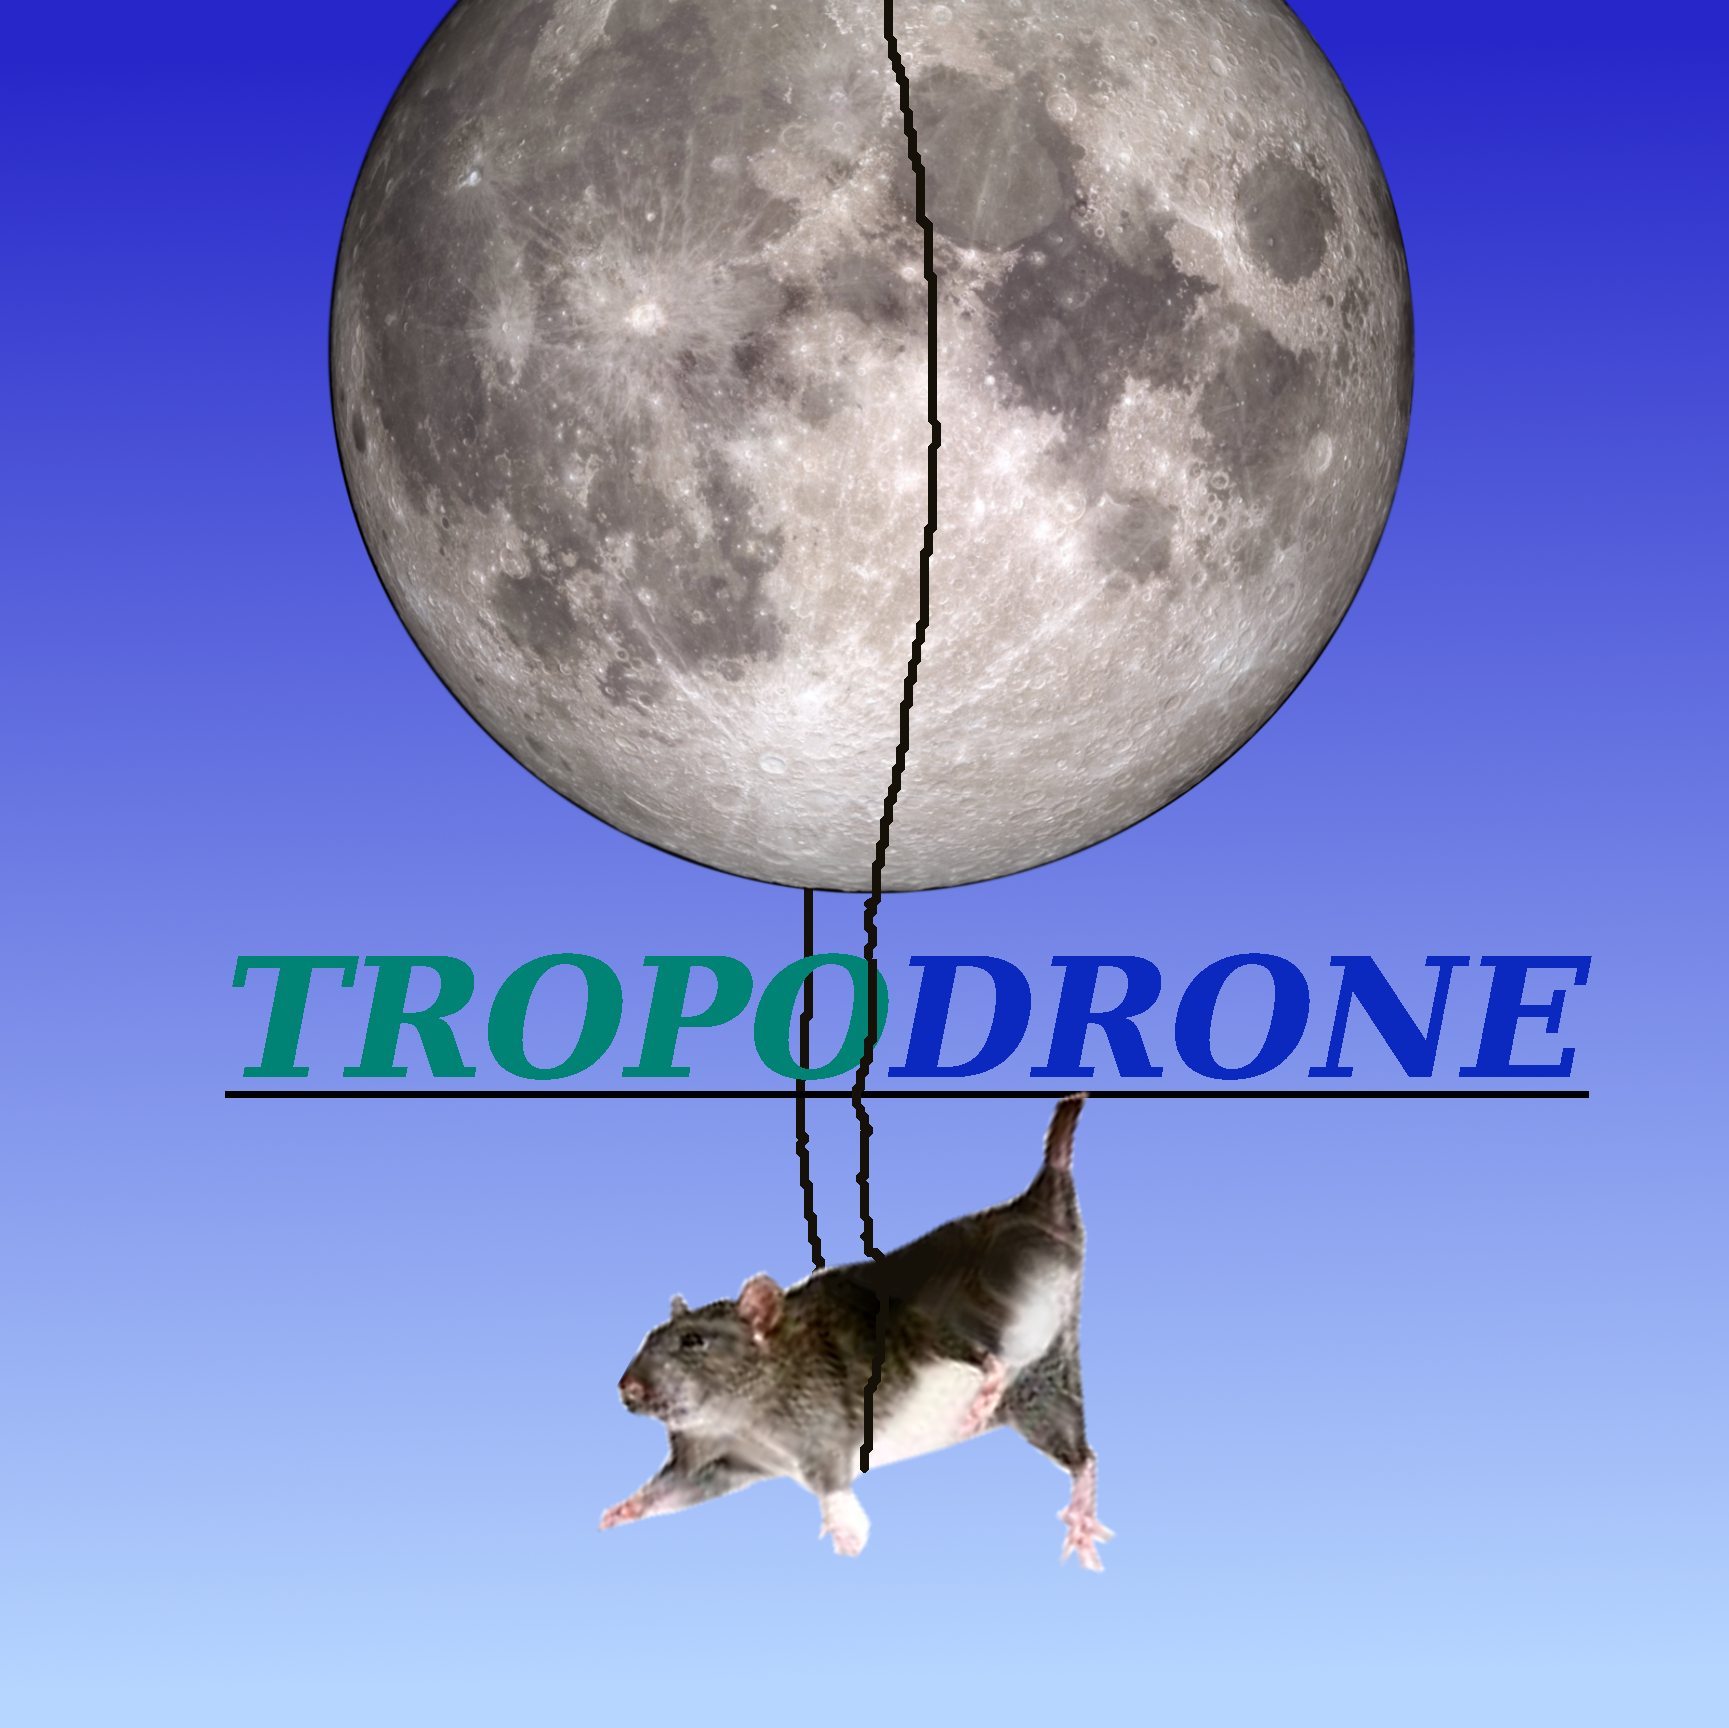
\includegraphics[width=15cm]{../Images/logo.png}
\end{center}


\end{Huge}

\clearpage

\tableofcontents

\clearpage

\section{Introduction}

\subsection{Besoins}
Notre projet part d'un constat: Les drones sont amenés à se développer fortement dans les années à venir, par exemple avec les services de livraison d'Amazon. Dans ce cadre, nous voulions apporter une amélioration significative pour répondre aux problématiques suivantes:
\begin{itemize}
	\item Autonomie: \\
		Les drones, particulièrement les drones quadricoptères de petite envergure possèdent une assez faible autonomie, ce qui réduit leur rayon d'action ainsi que la charge utile qu'ils peuvent supporter.
	\item Sécurité: \\
		Les drones sont des dangers, pour eux mêmes comme pour leur environnement. Les drones peuvent souffrir de problèmes techniques (comme la perte de batterie) et tomber en vol. On devine les dangers inhérents à ce genre de situation. De plus, les drones rentrent parfois dans des obstacles, et les dégâts peuvent vite revenir cher.
\end{itemize}

\subsection{Notre projet}
Notre projet part de ces constats pour aboutir à une solution, novatrice, qui n'a pas de concurrence sur le marché~: proposer aux pilotes amateurs et aux industriels un hybride entre un drone et un petit dirigeable à travers une structure qui permette d'augmenter un petit drone quadricoptère de 25 cm d'envergure.

\subsection{Contraintes}
Nous avons défini des besoins, de ces besoins découlent des contraintes. Ces contraintes sont:
\begin{itemize}
	\item Autonomie~:
		\begin{itemize}
			\item Du drone~:\\
			Avoir une autonomie supérieure à celle du drone, avec comme sans charge utile.
			\item Des ballons~:\\
			Avoir des ballons "étanches" à l'hélium, c'est à dire qui le retiennent au moins trois jours avec des pertes de l'ordre de 30\%.
		\end{itemize}
	\item Sécurité~:
		\begin{itemize}
			\item Structure~:\\
				Faire une structure qui enveloppe le drone et le protège des chocs.
			\item Sustentation~:\\
				Éviter que le drone ne tombe de manière dangereuse en cas de problème technique.
		\end{itemize}
	\end{itemize}
	Afin que le drone reste manœuvrable malgré sa structure, nous nous sommes également fixé des contraintes de manœuvrabilité~:
	\begin{itemize}
		\item Maneuvrabilité~:
			\begin{itemize}
				\item Retenir le drone~:\\
					La structure doit entacher au minimum les déplacements possibles du drone, en rotation comme en translation.
				\item Navigation~:\\
					Le drone doit pourvoir naviguer sur un intervalle de 15 mètres de hauteur.
			\end{itemize}
	\end{itemize}

\subsection{Applications}
Pour répondre à ses contraintes, nous avons mis en place ces solutions:
\begin{itemize}
	\item Ballons~:\\
		Nous utilisons trois ballons de 25m3 de contenance pour retenir le poids d'un drone de 750g, ce qui permet de très fortement ralentir sa chute.
	\item Structure~:
		\begin{itemize}
			\item Les ballons sont positionnés de sorte que leur centre de gravité coïncide avec celui du drone, pour plus de stabilité~;
			\item Le drone est relié à la structure par deux fils, ce qui lui laisse une grande liberté de mouvements~;
			\item Les ballons, disposés autour du drone, le protègent des chocs.
		\end{itemize}
\end{itemize}


\subsubsection{Légalité}
Faute de juridiction quant aux appareils volants de ce type, nous nous sommes rabattus sur les contraintes légales imposées aux drones et aux ballons séparément.\\
\begin{itemize}
	\item Notre drone est de catégorie A (- de 25 kg)~:\\
		Il n'est soumis à aucune contrainte qui nous limiterait dans le choix de nos solutions techniques, ou qui limiterait nos objectifs.
		Cependant, nous restons soumis aux mesures de sécurité élémentaires (ne pas trop s'approcher durant la phase de décollage et d'atterrissage, ne pas survoler les terrains militaires...).
	\item Le ballon entre dans la catégorie « léger »~:\\
		La ficelle supportant la charge utile doit casser au-dessous de 23 kg.
		Suite à des tests, la ficelle qui servira à tenir nos ballons se rompt à une tension comprise entre 15 et 20 kg.
\end{itemize}

\subsubsection{Drone}
	Caractérisitques du drone XCSOURCE en prenant en compte les hélices~: \\
	\begin{itemize}
		\item 290 mm diagonale~;
		\item 190 mm longueur~;
		\item 70 mm hauteur~;
		\item moteur EMAX MT2204 2300KV Brushless Motor~;
		\item 450 g.
	\end{itemize}
	\begin{center}
		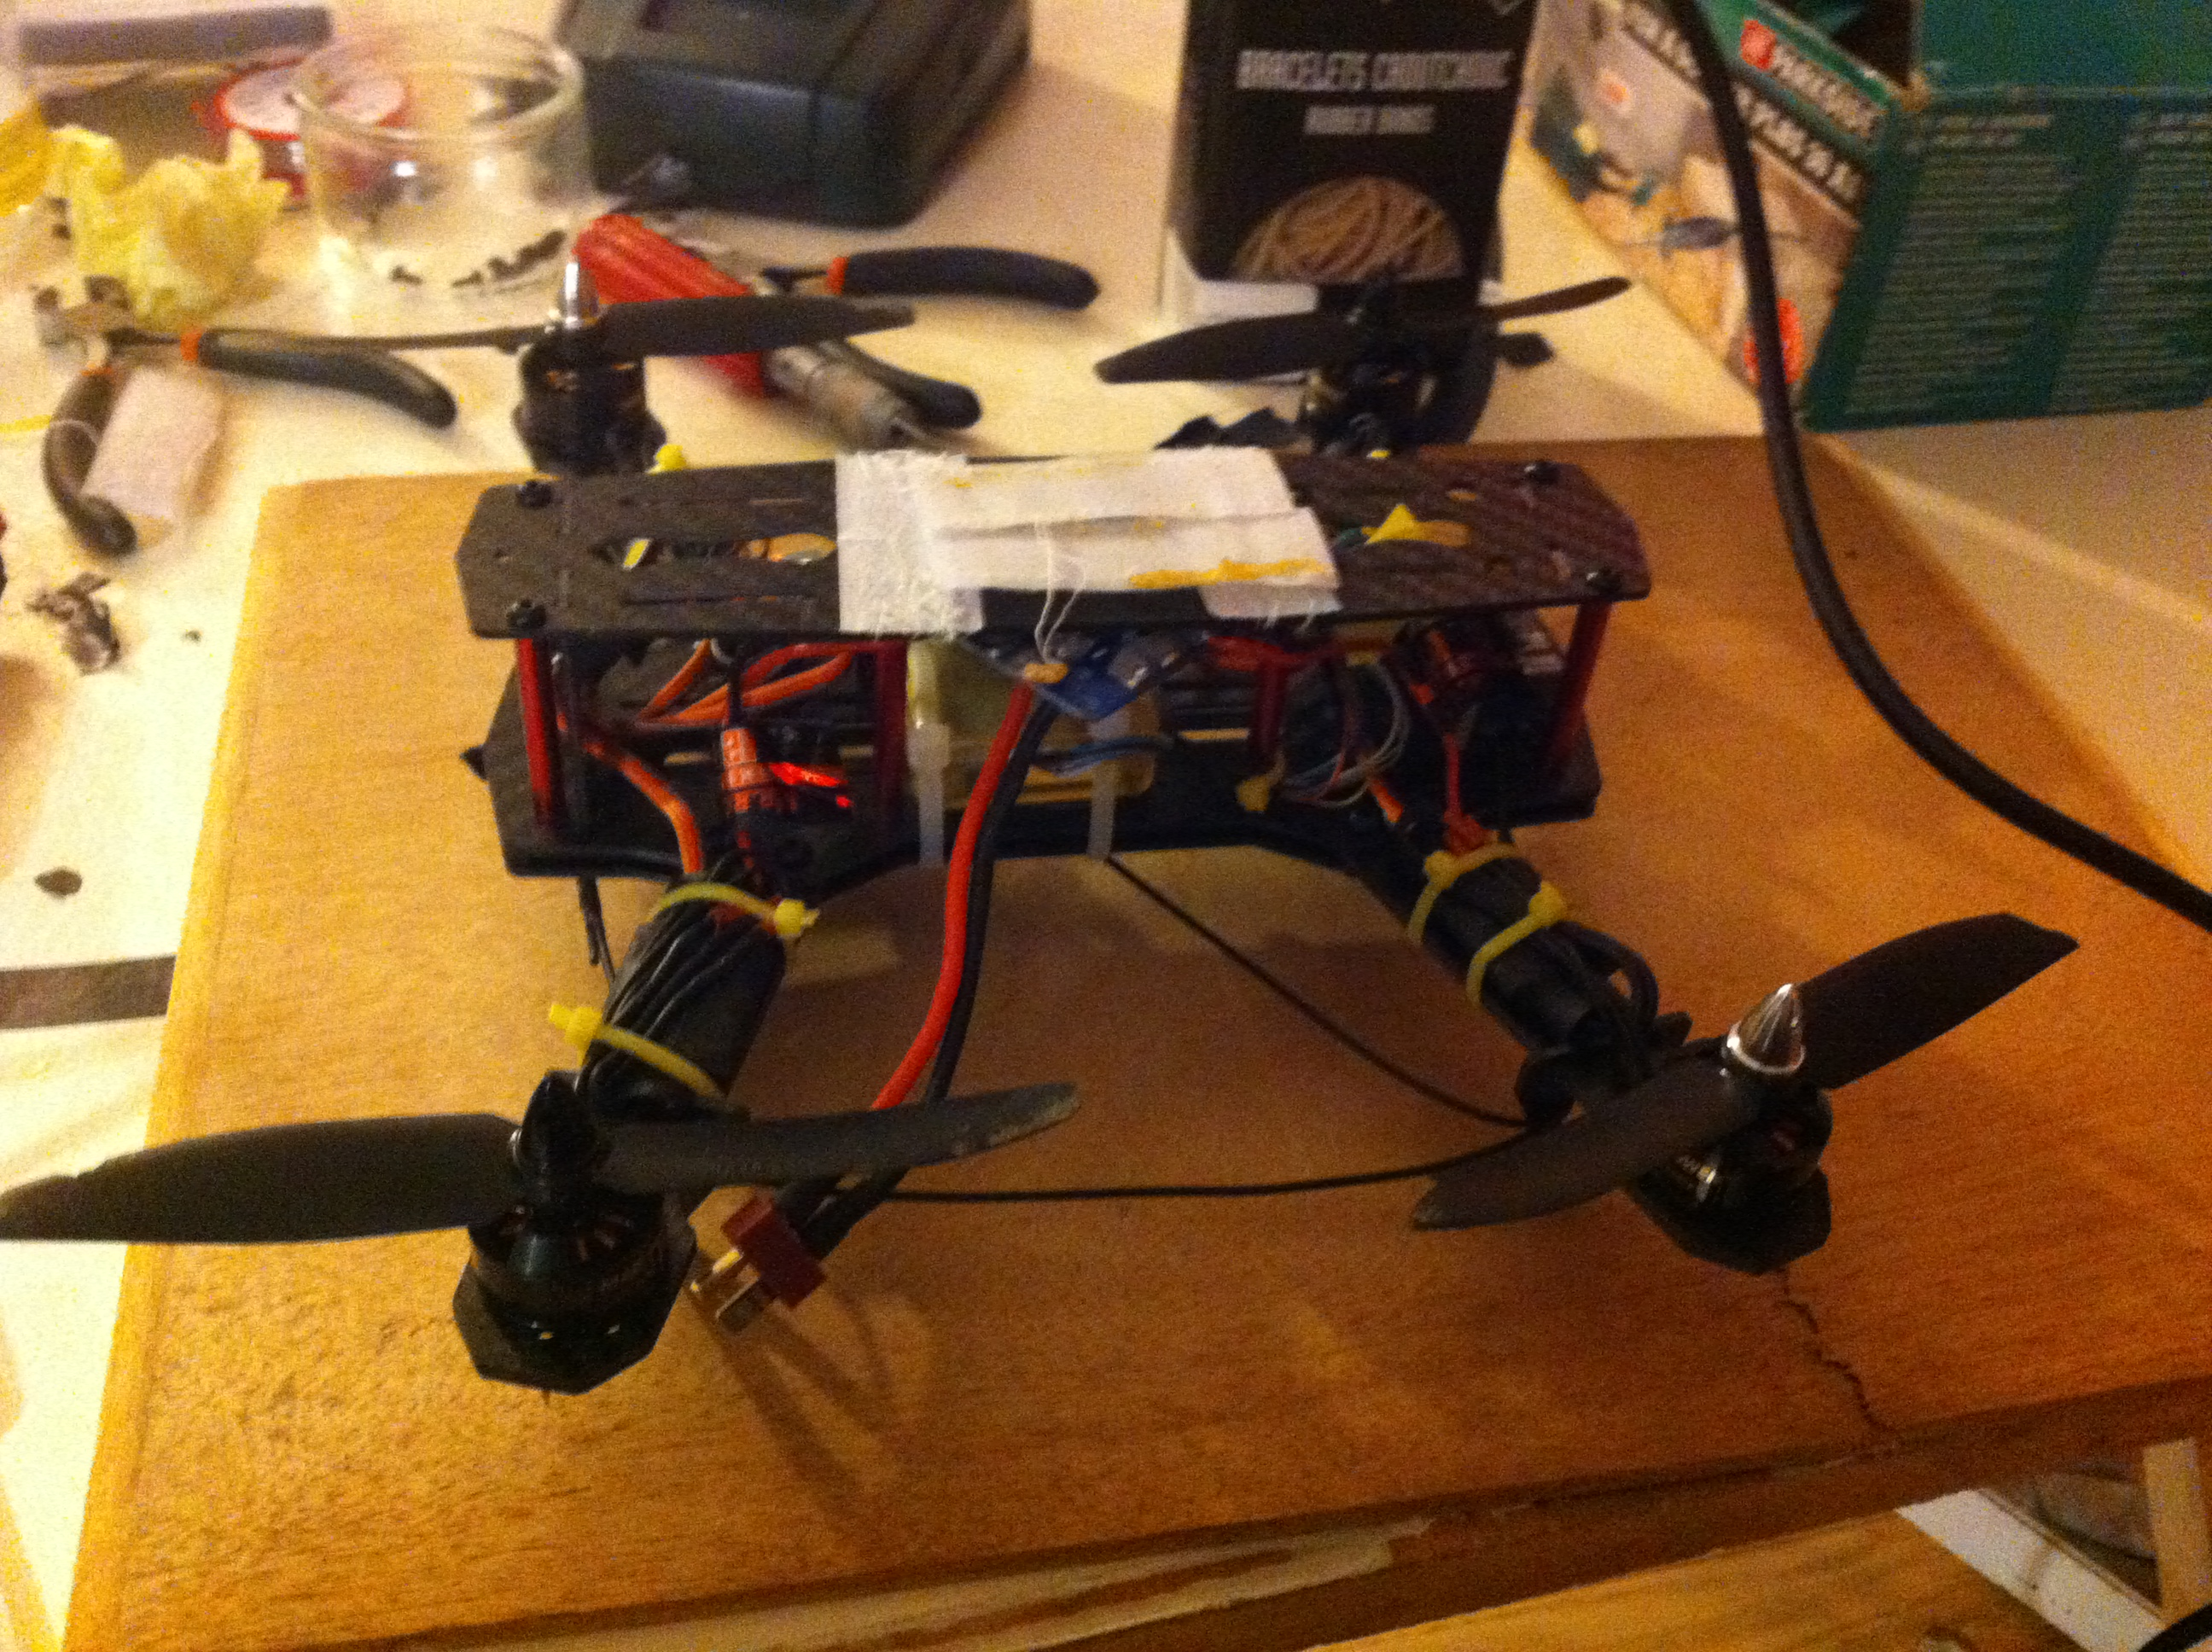
\includegraphics[width=6cm]{../Images/drone.JPG}
	\end{center}
	\captionof{figure}{Drone XCSOURCE.}

\paragraph{Caractéristiques moteur}

Les moteurs sont des brushless triphasé de 2300 KV alimenté en 12 V avec une consommation nominale de 7.5 A, soit 90 W. Leur rendement est de 0.9.

\paragraph{Capacité de levage}

La capacité de levage dépend du nombre d'hélice du diamère des hélices, du pas des hélices et de la vitesse de roation des moteurs.

\begin{center}
 $Puissance(N) = P \times D^3 \times RPM^2  \times 10^{-10} \times 10^{-3}$
\end{center}

Où P est le pas en inch, D le diamètre en inch, et RPM la rotation par minute.

\paragraph{Batterie du drone}

Ci dessous les caractérisitques de la batterie~:
\begin{itemize}
		\item Lithium Polymère~;
		\item Masse 135g~;
		\item Capacité 1800mAh~;
		\item 25C , soit 45 A max en continu~;
		\item 11.1V en 3S~;
		\item 135 g~;
		\item Rapport poids puissance : 148Wh/Kg.
\end{itemize}


\paragraph{Autonomie}

Le calcul théorique de l'autonomie est le suivant~:

\begin{center}
 $Power = P \times D^4 \times RPM^3 \times 5.33 \times 10^{-15}$ \\
 $Thrust = P \times D^3 \times RPM^2 \times 10^{-10} \times 10^{-3}$
\end{center}

Où Power est la puissance en W fournie, Thrust le levage en N, P le pas des hélices en inch, RPM la vitesse de roation en $tr.min^{-1}$, D le diamètre des hélices en inch.

Ainsi pour soulever 115 g par moteur, il faut consommer 11,2W. Le total est de 44,8W instantanées soit une autonomie théorique de $(11 \times 1,8 \times 3600)/44,8 = 1735$s ou 28 min.
En partique 18 A sont consommés en instantané $(1,8 \times 3600)/18 = 360$ secondes d’autonomie soit 6 min. Nous pouvons conclure que le modèle théorique ignore de très nombreux paramètres influençant la consommation des moteurs.

\section{Ballon}

\subsection{Élévation}

Le Tropodrone doit utiliser un moyen de supporter une partie du poids du drone sans dépenser d'énergie dans le but d'augmenter l'autonomie du drone en le permettant de faire tourner ses hélices à un régime plus faible. Pour ce faire nous utilisons la poussée d'Archimède d'un gaz plus léger que l'air. Comme ce gaz est plus léger que l'air la somme de son poids et de sa poussée d'Archimède forment une force verticale orientée vers le haut.

\subsubsection{Archimède}

La poussée d'Archimède est définie par~:

\enquote{Tout corps plongé dans un fluide au repos, entièrement mouillé par celui-ci ou traversant sa surface libre, subit une force verticale, dirigée de bas en haut et opposée au poids du volume de fluide déplacé ; cette force est appelée poussée d'Archimède.}

\begin{figure}[H]
	\centering
	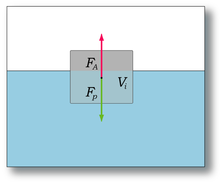
\includegraphics[width=5cm]{../Images/pousse_archimede.png}
	\caption{Représentation de la poussée d'Archimède}
\end{figure}

Cette force se calcule grâce à la formule~:

\begin{center}
  \boxed{\vv{Fa} = -M_F \times \vv{g}}
\end{center}

Où $\vv{Fa}$ est la poussée d'Archimède en $N$, $M_F$ la masse du fluide contenue dans le volume déplacé en $kg$, $\vv{g}$ la valeur du champ de pesanteur en $N.kg^{-1}$. \\

Un ballon de gaz est donc soumis à deux forces~: son poids et sa poussée d'Archimède~:

\begin{center}
  \boxed{\vv{F_{ballon}} = \vv{P_{ballon}} + \vv{Fa_{ballon}}}
\end{center}

Où $\vv{F_{ballon}}$ est la force d'élévation du ballon en $N$, $\vv{P_{ballon}}$ le poids du ballon en $N$, $\vv{Fa_{ballon}}$ la poussée d'Archimède exercée sur le ballon en $N$. \\

Nous pouvons remarquer que si $P_{ballon} < Fa_{ballon}$ alors il existe une force d'élévation orientée vers le haut. De même cette force sera toujours plus petite que la poussée d'Archimède exercée sur le ballon, car le ballon et le gaz possèdent toujours une masse~: $F_{ballon} < Fa_{ballon}$.
Par la suite nous appellerons capacité d'élévation la masse que peut soulever la force d'élévation d'un ballon~:
\begin{center}
	\boxed{Ca_{ballon} = \frac{F_{ballon}}{g}}
\end{center}

Où $Ca_{ballon}$ est la capacité d'élévation en $kg$, $F_{ballon}$ la force d'élévation en $N$ et $g$ la valeur du champ de pesanteur en $N.kg^{-1}$.

\subsubsection{Gaz}

Pour avoir un gaz plus léger que l'air il faut qu'il possède une masse volumique inférieur à celle de l'air~: $1.29kg.m^3$. Plusieurs gaz remplissent cette condition, les plus courants sont l'hélium est l'hydrogène dont les masses volumiques et les capacités d'élévation calculées sont~:

\begin{center}
	\begin{tabular}{|l|c|c|c|}
		\hline
		Gaz & Air & Hydrogène & Hélium \\
		\hline
		Masse Volumique $(kg.m^3)$ & 1.29 & 0.08988 & 0.1785 \\
		\hline
		Force d'élévation $(N.m^3)$ & 0 & 11.77 & 10.90 \\
		\hline
	\end{tabular}
\end{center}

Le gaz retenu et l'hélium car il ne présente pas de risque de combustion contrairement à l'hydrogène, même si sa masse volumique est plus importante et qu'il est plus difficile à trouver.

\subsubsection{Dilatation}

En prenant exemple sur les montgolfières nous avons cherché à connaitre le gain de volume que pourrait avoir l'hélium à une température élevée. Ce gain de volume apporte directement une réduction de la masse volumique et donc l'augmentation de la force d'élévation.

La loi de Charles permet de calculer la dilatation d'un gaz. D'après Charles il existe un rapport volume température constant dépendent seulement de la pression du gaz et de la quantité de matière du gaz étudié.

\begin{center}
 \boxed{\displaystyle{\frac{V_1}{T_1} = \frac{V_2}{T_2} = f(P, n)}} \\
 $\displaystyle{V_3 = f(P, n) \times T_3}$
\end{center}

Où $V_n$ est le volume du gaz en $m^3$ à la température $T_n$ en $K$, $P$ la pression du gaz en $Pa$, $n$ la quantité de matière en $mol$ et $f(P, n)$ le rapport constant entre volume et temperature en $m^3.K^{-1}$.

L'application de cette loi à l'hélium à une température de $200 \degree C $ donne les résultats suivants~: \\

Le volume molaire de l'hélium est~: $22.414\times 10^{-3} m^3.mol^{-1}$ à $273.25K$. \\

\begin{center}
	$\displaystyle{f(P, n) = \frac{22.414\times 10^{-3}}{273.25} = 8.2\times 10^{-5} m^3.mol^{-1}.K^{-1}}$
	\bigbreak
	$T_{200} = 200 \degree C = 473.25K$
	\medbreak
	$\displaystyle{V_{T_{200}} = 8.2\times 10^{-5} \times 473.25 = 38.811 \times 10^{-3}} m^3.mol^{-1}$
\end{center}

Donc à $200 \degree C$ l'hélium a un volume molaire de $38.811 \times 10^{-3} m^3.mol^{-1}$ équivalent à 1.59 fois son volume molaire d'origine. Malgré cette augmentation de volume, la force d'élévation varie peu car le poids de l'hélium est très faible et que la réduction de celui ci ne fera que se rapprocher de la valeur de la poussée d'Archimède~: \\

\begin{center}
  $\displaystyle{F_{T_0} = Fa_{air} - P_{helium} = 10.90 N}$
  \bigbreak
  $\displaystyle{F_{T_{200}} = Fa_{air} - \frac{P_{helium}}{1.59} = 11.57 N}$ \\
\end{center}

$F_{T_{200}} = 1.06 \times F_{T_0}$

À cause des faibles résultats obtenus et des problèmes introduits par la mise en œuvre du chauffage d'un gaz~: résistance de l'enveloppe du ballon~; résistance de chauffage~; alimentation de la résistance. Cette idée est donc abandonnée.

\subsection{Enveloppe}

\subsubsection{Matériaux}

Lors de la sélection des matériaux à utiliser pour l'enveloppe des ballons nous avons cherché les matériaux déjà utilisés dans le domaine des ballons dirigeables et des sondes. Le plus utilisé est le latex mais celui ci ne se trouvait qu'en forme de ballon sphérique (ballon de baudruche) ce qui empêche tout contrôle de la forme.

Ci dessous sont listés les matériaux comparés lors de notre choix~:

\begin{center}
\begin{tabular}{|p{0.2\linewidth}|p{0.35\linewidth}|p{0.35\linewidth}|}
		\hline
		Matériaux & Avantages & Inconvénients \\
		\hline

		\rowcolor{OrangeT}
		Latex &
		Facile à trouver dans le commerce &
		Seulement en forme sphérique~; peu étanche \\
		\hline

		\rowcolor{RedT}
		Hypalon & Étanche & Introuvable dans le commerce~; fragile aux ultraviolets \\
		\hline

		\rowcolor{GreenT}
		Mylar (PET) &
		Facile à trouver dans le commerce~; résistant à la traction~; peut être assemblé~; léger~: $17 g.m^{-2}$ &
		Raide~; fragile au cisaillement et à la perforation \\
		\hline

		\rowcolor{RedT}
		Chloroprène &
		& Introuvable dans le commerce \\
		\hline

		\rowcolor{RedT}
		Butyle &
		& Introuvable dans le commerce \\
		\hline
\end{tabular}
\end{center}

Le matériau retenue et le polyéthylène téréphtalate (PET) ou de nom commercial Mylar. Ce matériaux est un polymère très léger et solide à la traction, mais il a aussi ses désavantages, il est fragile à la perforation et comme la plupart des polyéthylène très difficile à coller.

Lors de nos tests d'assemblage nous avons utilisé du PET provenant de couvertures de survie car peu chers, mais après quelques tests d'étanchéité nous mettons clairement en doute la qualité du PET des couvertures de survie. D'autre sources de PET sont possibles notamment dans les films alimentaires, un exemple et le Mylar 850, mais malgré sa très grande qualité affichée (perméabilité, épaisseur, masse) celui ci ne se vend qu'en bobine de 2500 mètres.

\subsubsection{Étanchéité}

L'étanchéité du PET est importante pour garder le gaz à l'intérieur des ballons et ainsi autoriser le drone à voler plus longtemps avec l'assistance des ballons. Pour ce faire une recherche théorique de la perméabilité du PET a été réalisée ainsi que des tests d'étanchéité à l'air.

Lors de l'assemblage des ballons de nombreux problèmes d'étanchéité ont été rencontré, plusieurs pistes étaient alors possibles~: le manque d'imperméabilité du matériau choisi ou des collages. Pour vérifier ces deux hypothèses, des tests ont été réalisé sur des ballons finis et sur de simples feuilles de PET sans assemblage et collage.


La perméabilité du PET a rapidement été mise en doute, en effet les feuilles que nous utilisions étaient d'une très faible épaisseur ($12\mu m$) et sa qualité était incertaine car nous utilisions du PET de couvertures de survie.

Plusieurs thèses étudiant la perméabilité des polymères au gaz comme l'hélium ont été trouvées mais le manque de valeurs pour l'épaisseur de notre film, la pression utilisée ou encore la température n'a pas permis un usage fiable de ces formules et de ces données.
Malgré tout nous pouvons expliquer la perméabilité du PET par son taux de cristallisation. Les cristaux étant considérés comme parfaitement imperméables, l'air ne peut passer que entre ces cristaux, donc l'épaisseur du film et le taux de cristallisation impactent directement la perméabilité du film.

Les seuls chiffres que nous possédons sont ceux d'un film de PET alimentaires le Mylar 850 déjà énoncées précédemment~:

\begin{center}
 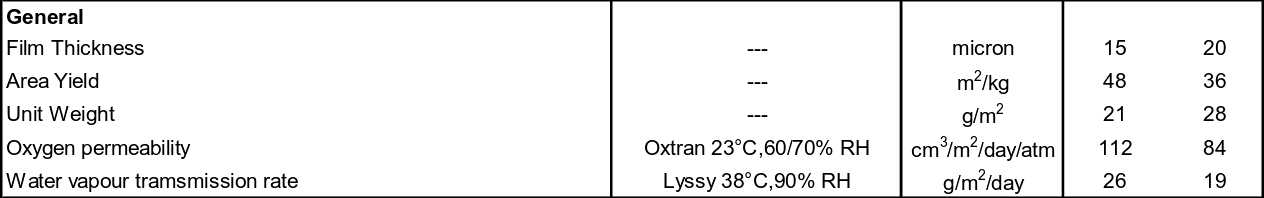
\includegraphics[width=15cm]{../Images/permeabilite.png}
\end{center}

Le film s'approchant le plus du notre et de $15\mu m$ ayant une fuite de 1.12L par $m^2$ de surface par jour et par atmosphère, 1 dans notre cas.

Sans rentrer dans les détails des calculs de perméabilité, nous sommes passés à des tests d'étanchéité à l'air, pour cela nous devons éliminer tout usage de collage même si nous pouvons dans l'absolu garantir leur étanchéité.
Nous avons alors créé une cloche maintenant une feuille de PET légèrement pliée pour rentrer dans la cloche, la cloche est percée sur le haut et plongée dans l'eau à l'aide de quelques masses. Enfin sur le haut de la feuille de PET nous disposons une petite masse d'environs 10g.
Le but de cette expérience est d'observer le passage de l'air à travers la feuille de PET, si l'air passe à travers la feuille alors la masse disposée au dessus tombera avec le temps, de plus l'eau permet de faire un très bon bouchon avec le bas de la cloche.

\begin{figure}[H]
	\centering
	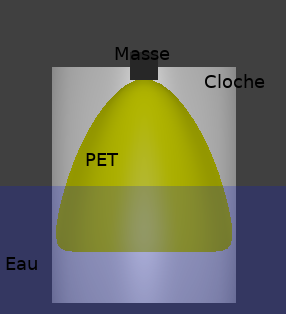
\includegraphics[width=7cm]{../Images/etancheite.png}
	\caption{Test d'étanchéité du PET, le PET est maintenu par la cloche dans l'eau, nous mesurons la chute de la masse disposée au dessus du PET.}
\end{figure}

Après avoir laissé l'ensemble dans l'eau pendant une semaine une très faible baisse de volume à pu être constatée mais rien ne pouvant justifier les fuites assez importantes des ballons assemblés.

\begin{figure}[H]
 \centering
 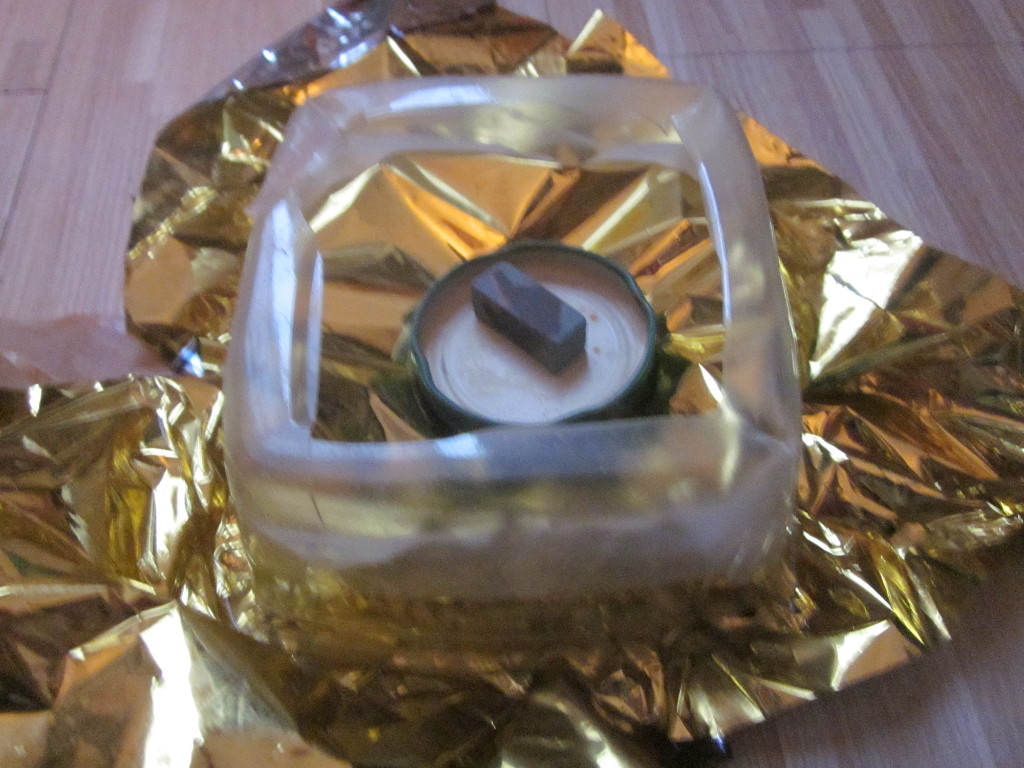
\includegraphics[width=7cm]{../Images/cloche_pet.JPG}
 \caption{Cloche utilisée pour tester l'étanchéité du PET.}
\end{figure}



Nous nous sommes alors penchés sur l’imperméabilité des jointures de collage, ainsi nous avons pu observer que le moindre pli lors du collage pouvait potentiellement créer une fuite, de plus un collage favorisant les contraintes de pelage avait tendance à déchirer le PET. Pour éviter ces fuites nous devons en plus d'une colle utilisée pour maintenir le PET utiliser un mastique pour boucher toutes les fuites. Le premier mastique choisi fut le latex car il avait l'avantage de toujours coller au PET comme certain adhésif en pâte. Malheureusement le latex était assez difficile à appliquer et il semble après des tests attaquer la colle utilisée plus aisément que l'eau. Nous l'avons alors remplacé par de la colle acrylique que nous trouvons pour les collages en décoration, cette colle a le fort avantage d'être épaisse et de ne pas se rétracter au séchage, ainsi nous pouvons boucher tout le volume d'un pli.

\begin{figure}[H]
 \centering
 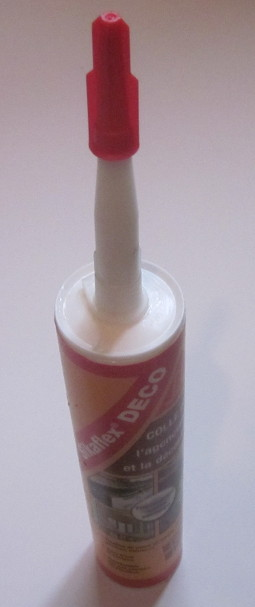
\includegraphics[width=3cm]{../Images/colle_acrylique.JPG}
 \caption{Colle acrylique utilisée pour boucher les fuites.}
\end{figure}


Les différentes méthodes d'étanchéification des jointures ont été testées de deux façons.
Premièrement deux triangles de PET sont découpés puis collés sur deux de leurs bords, l'ensemble forme ainsi un cône que nous pouvons tester de la même manière que le PET seul avec une cloche plongée dans l'eau.
Deuxièmement un ballon est assemblé avec la méthode d'étanchéification étudiée, le ballon est gonflé à une pression moyenne et de l'eau savonneuse est passée autour de l'enveloppe extérieur du ballon, ainsi la moindre bulle nous signale une fuite, nous pouvons faire de même en plongeant le ballon dans l'eau. Malheureusement ce dernier test compromet les résultats car l'eau a tendance à boucher les fuites par sa viscosité, c'est ainsi que nous pouvons remarquer que nos ballons les plus étanches présentent toujours des fuites car nous constatons une baisse de volume mais sans pouvoir détecter la moindre bulle d'air au savon ou en plongeant le ballon dans l'eau.


\begin{figure}[H]
 \centering
 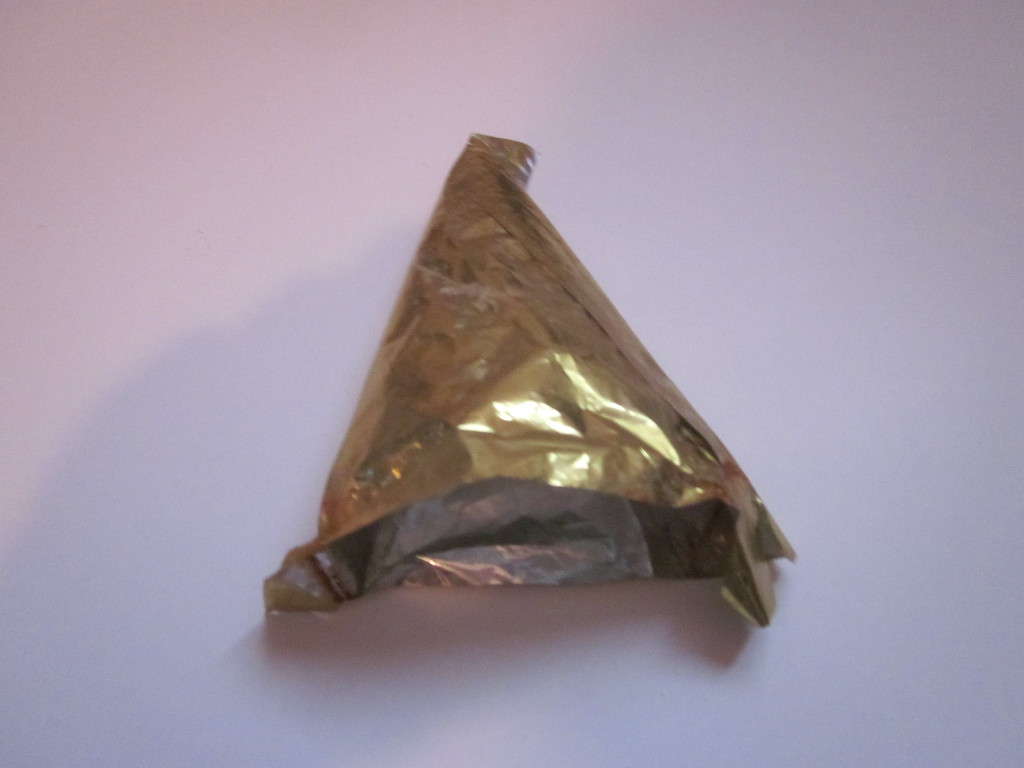
\includegraphics[width=7cm]{../Images/cloche_colle.JPG}
 \caption{Cloche utilisée pour tester l'étanchéité des collages.}
\end{figure}

\begin{figure}[H]
 \centering
 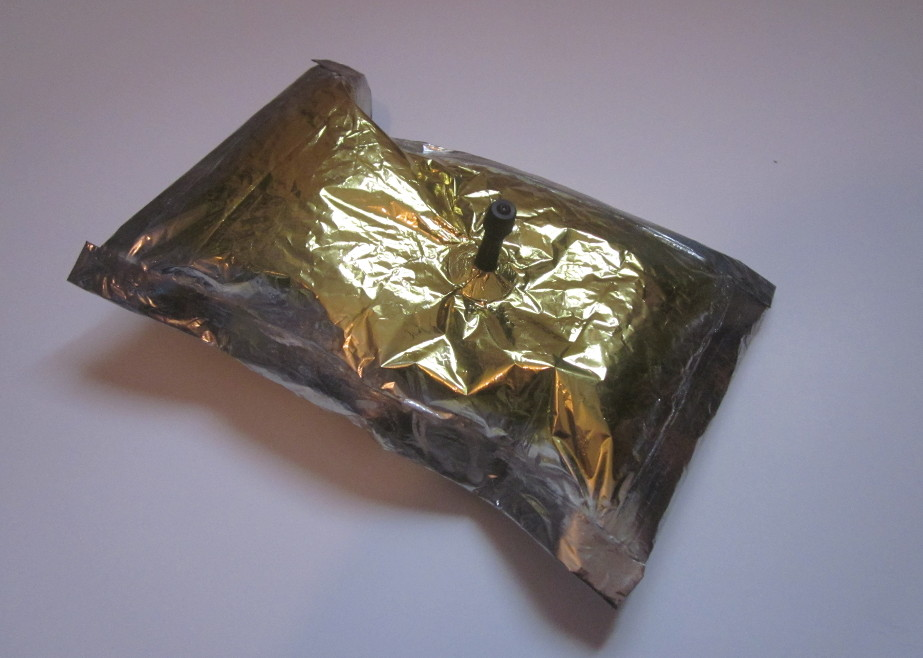
\includegraphics[width=10cm]{../Images/ballon_etanche.JPG}
 \caption{Ballon de test d'étanchéité, formé de deux feuilles de PET.}
\end{figure}


\subsection{Collage}

Une fois le patron du ballon découpé sur une feuille de PET, nous devons coller les jointures prévues à cette effet. Nous utilisons un collage au lieu d'un thermo-collage car ce dernier est plus compliqué à mettre en œuvre, en effet le thermo-collage nécessite un appareil spécifique et il produit de très mauvaises jointures si la feuille de PET est froissée, là où la colle pourrait agir comme un mastique.

Comme nous l'avons précédemment expliqué le PET est un matériau très difficilement collable, en contrepartie de nombreuses colles ont été testées avec au final bien plus de colles inefficaces qu'utilisables.

Ci-dessous l'ensemble de colles testées~:

\begin{center}
  \begin{tabular}{|p{0.3\linewidth}|p{0.3\linewidth}|p{0.3\linewidth}|}
		\hline
		Colle & Avantages & Inconvénients \\
		\hline

		\rowcolor{OrangeT}
		Néoprène (Polychloroprène) &
		Étanche, élastique, adhèrent &
		Difficile à appliquer \\
		\hline

		\rowcolor{OrangeT}
		406 (cyanoacrylate d'ethyle) et 770 (primaire) &
		Adhèrent, rigide, facile à appliquer &
		Fragile à l'eau \\
		\hline

		\rowcolor{GreenT}
		401 (cyanoacrylate d'ethyle) et 770 (primaire) &
		Très adhèrent, rigide, facile à appliquer &
		Fragile à l'eau \\
		\hline

		\rowcolor{RedT}
		330 et activateur &
		Élastique &
		Peu adhèrent \\
		\hline

		\rowcolor{RedT}
		Polyester &
		Polymérisation avec catalyseur &
		Peu adhèrent \\
		\hline

		\rowcolor{RedT}
		Polyuréthane &
		& Peu adhèrent \\
		\hline

		\rowcolor{RedT}
		Acétone &
		& Peu adhèrent \\
		\hline

		\rowcolor{RedT}
		Vinylique &
		Facile à appliquer &
		Peu adhèrent, temps de séchage trop long \\
		\hline

		\rowcolor{RedT}
		Acrylique &
		Facile à appliquer &
		Peu adhèrent \\
		\hline
  \end{tabular}
\end{center}

La colle retenue est la cyanoacrylate d'éthyle ou 401, cette colle est une des plus adhérentes au PET, elle a un temps de séchage assez court et surtout ne dépend pas d'une polymérisation à l'air mais à l'eau de surface, en effet les feuilles de PET étant très imperméables le temps de séchage pour une colle polymérisé à l'air peu prendre plusieurs heures, certaine ne sèchent presque jamais comme la colle vinylique.

Les jointures de collage sont collées par l'extérieur pour pouvoir ajuster sans difficulté les deux bordures. Malheureusement ce collage extérieur contraint la colle à un pelage, cette contrainte étant la pire pour la majorité des colles.

\subsubsection{Résistance}

Les différentes contraintes d'un collages sont décrites dans le tableau suivant~:
\begin{center}
 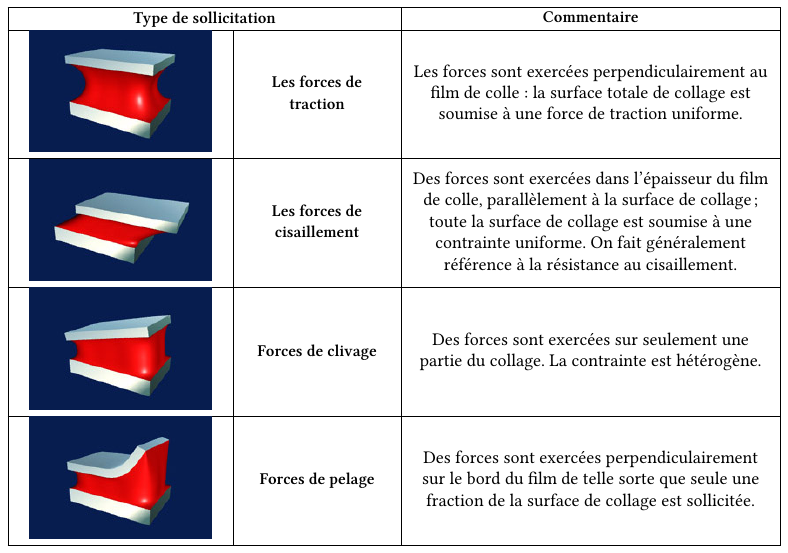
\includegraphics[width=15cm]{../Images/colle_contraintes.png}
\end{center}

La contrainte de pelage ici est la pire car elle exerce le maximum d'effort sur un très petite zone de collage ce qui amène à un déchirement du collage qui fragilise les zones voisines de collage. Pour remédier à ce problème, il faut changer de type de contrainte, dans notre cas passer d'un pelage à un cisaillement. Ceci est réalisable en collant la jointure sur l'un des côtés du ballon, formant ainsi un collage plat au lieu d'une forme en T.

\begin{figure}[H]
	\centering
 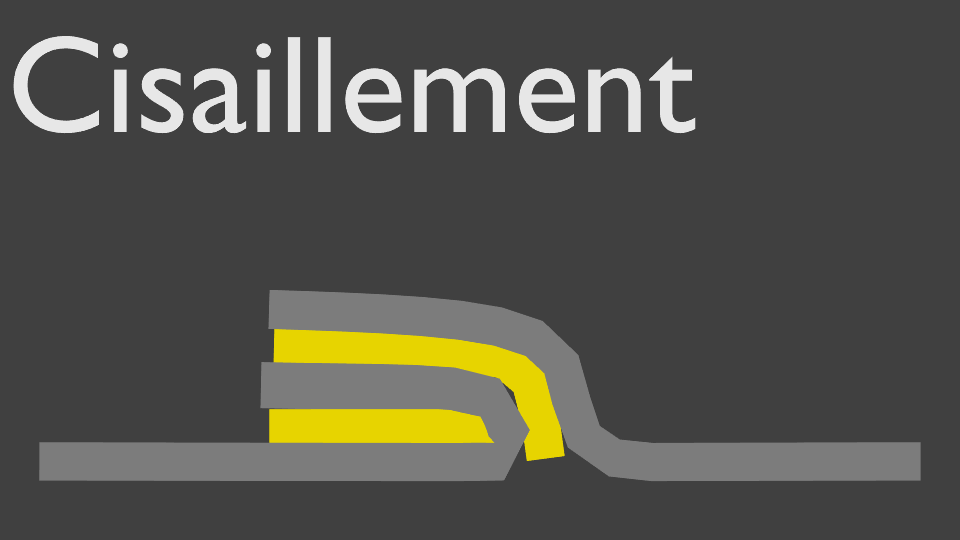
\includegraphics[width=7cm]{../Images/colle_cisaillement.png}
 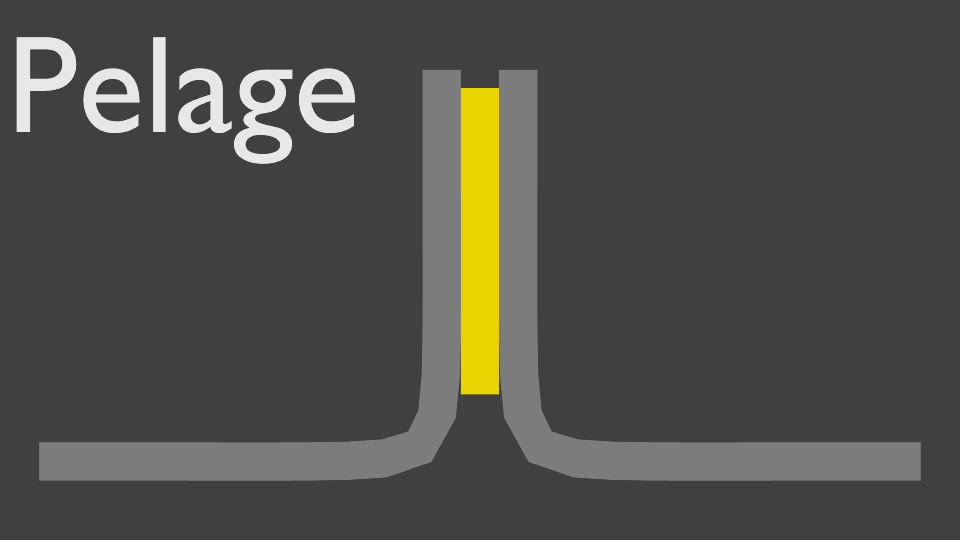
\includegraphics[width=7cm]{../Images/colle_pelage.png}
 \caption{À gauche le schéma d'un collage favorisant les contraintes de pelage, à droite le schéma d'un collage favorisant les contraintes de cisaillement.}
\end{figure}

Deux tests de traction ont alors été réalisés en pressant et collant deux feuilles de PET dans des planches en bois servant de support à la traction, ensuite les deux feuilles de PET étaient collées entre elles avec chacune des techniques de collage.

\begin{figure}[H]
	\centering
 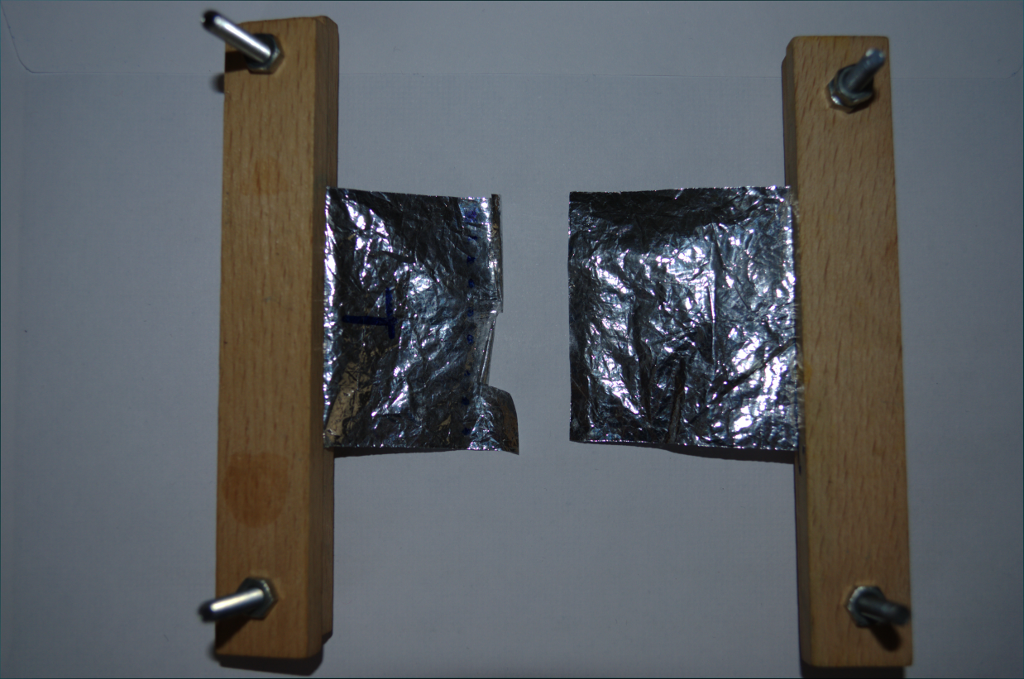
\includegraphics[width=7cm]{../Images/test_pelage.png}
 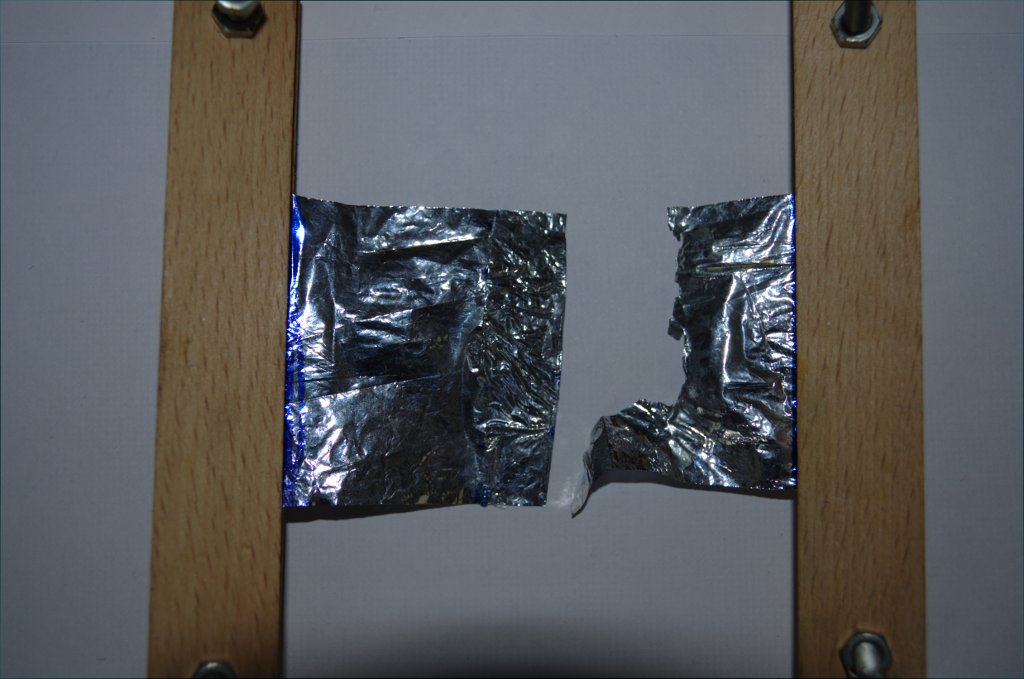
\includegraphics[width=7cm]{../Images/test_cisaillement.png}
 \caption{À gauche la photo après la contrainte de pelage, remarquons la rupture du substrat par déchirement et la rupture de la colle, à droite la photo après la contraintes de cisaillement, remarquons la seul rupture du substrat après étirement de la feuille de PET.}
\end{figure}

Lors de ces tests nous pouvons remarquer que la contrainte de pelage a tendance à créer une rupture du substrat par le déchirement du PET et une rupture de la colle, celle ci se brise en restant sur un des deux côtés du substrat.
En ce qui concerne le test favorisant le cisaillement, il y a rupture du substrat mais cette fois ci avec un étirement de la feuille avant son déchirement, ainsi le collage reste intact.

Les mesures de forces lors des test de tractions sont présentes ci dessous~:

\begin{center}
  \begin{tabular}{|c|c|}
    \hline
    Pelage & Cisaillement \\
    \hline
    $0.45 N.cm^{-2}$ & $12.1 N.cm^{-2}$ \\
    \hline
  \end{tabular}
\end{center}

Nous remarquons que le collage a une résistance à la traction 27 fois supérieur si l'on favorise une contrainte de cisaillement au lieu d'une contrainte de pelage.
De plus les données constructeur de la colle indiquent une résistance au cisaillement de 7 à 11 $N.mm-2$ ce qui est largement supérieure au 0.12 $N.mm-2$ des tests, ce qui laisse penser que seul le PET est limitant dans la résistance des collages actuellement.


Cette technique de collage sera retenue pour l'assemblage de tous les futurs ballons.

\subsection{Forme}

Le Tropodrone est composé de trois ballons de taille identique dans le but d'avoir un centre de gravité confondu entre le drone et la structure, ce choix sera détaillé dans la partie montrant la conception de la structure.
La disposition la plus optimisée pour trois ballons est en triangle autour du drone, les ballons ressembleront donc à des parallélépipèdes avec deux pyramides à chacun de leurs sommets pour assurer une jointure entre les ballons.

\begin{figure}[H]
	\centering
 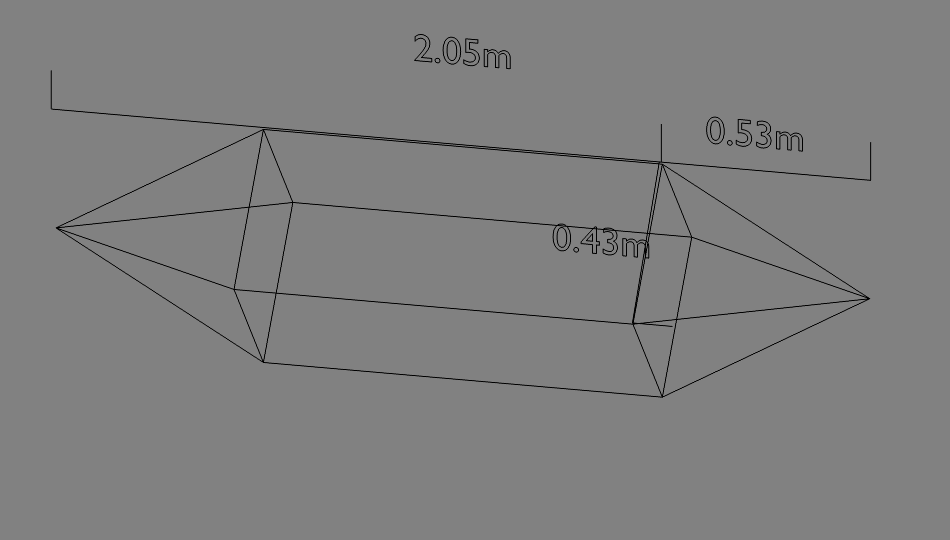
\includegraphics[width=12cm]{../Images/ballon.png}
 \caption{Vue d'ensemble d'un ballon.}
\end{figure}

\subsubsection{Calcul de la forme}

D'après le bilan maximal des masses il faudrait contenir $0.75m^3$ d'hélium dans l'ensemble des ballons. Nous partons donc de l'équation du volume pour retrouver les dimensions du ballon, heureusement des contraintes sont déjà présentes~:

\begin{itemize}
 \item la longueur du parallélépipède central est de 1m~;
 \item l'angle entre les arrêtes du sommets de la pyramide et la base de la pyramide est de $60 \degree$~;
 \item les ballons ont une orientation horizontale de $45 \degree$~;
 \item le volume du ballon est de $0.25m^3$.
\end{itemize}

\bigbreak

Pour $b$ la largeur du ballon, la formule du volume d'un ballon se compose du volume d'un parallélépipède d'un mètre~:

\begin{center}
 \boxed{V_{pa} = b^2}
\end{center}

Les deux pyramides ont un angle de $60 \degree$, leur hauteur est donc~: $\displaystyle{h = bidiagonale \times \tan{\frac{\pi}{3}}}$, où $\displaystyle{bidiagonale = \frac{\sqrt{b^2 \times 2}}{2}}$ la moitié de la diagonale de la base de la pyramide. \\
Le volume d'une pyramide est donc~:

\begin{center}
 \boxed{V_{py} = b^2 \times \frac{h}{3}}
\end{center}

La formule du volume d'un ballon est la suivante~:

\begin{center}
	\boxed{\displaystyle{V = 2(\frac{\sqrt{2 \times b^2}}{2} \times \tan \frac{\pi}{3} \times \frac{1}{3} \times b^2) + b^2}} \\
\end{center}

Nous simplifions la formule jusqu'à trouver un polynome nous facilitant la résolution pour une valeur nulle~:

\begin{center}
  $\displaystyle{V = \frac{\sqrt{6}}{3} \times b^3 + b^2 }$ \\
  $\displaystyle{b^3 \frac{\sqrt{6}}{3} + b^2 - 0.25 = 0}$
\end{center}

Malheureusement ce polynôme est du troisième degré, nous ne pouvons pas le résoudre aussi facilement qu'un polynôme du second degré, la méthode la plus simple dans notre cas est d'utiliser le théorème des valeurs intermédiaires, notre fonction de volume est croissante, continue et passant par zéro.

\begin{tikzpicture}[scale=1.5]
  \begin{axis}[
		domain=-0.1:.6,
    xlabel=$b$,
    ylabel={$V = 2(\frac{\sqrt{6}}{3} \times b^3) + b^2$},
    ytick={0, 0.25, 0.5, 0.75},
    xtick={0, 0.25, 0.43, 0.5}
  ]
		\addplot {((sqrt(6)/3) * x^3) + x^2};
		\draw (axis cs:-0.1,0.25) -- (axis cs:0.43,0.25);
		\draw (axis cs:0.43,0) -- (axis cs:0.43,0.25);
\end{axis}
\end{tikzpicture}


\paragraph{Résolution par bissection}

Pour trouver la largeur souhaitée pour un volume de $0.25m^3$ nous utilisons une résolution par bissection exécutée par un programme python. Une bissection est une méthode échantillonnant une fonction continue croissante ou décroissante dans un intervalle donné. Pour chaque intervalle un échantillon de la valeur intermédiaire est calculé, si sa valeur est supérieure à la valeur souhaitée, la borne supérieure de l'intervalle est réduite jusqu'à la valeur intermédiaire, dans la cas contraire où la valeur intermédiaire est plus petite que la valeur souhaitée, la borne inférieure de l'intervalle est augmentée jusqu'à la valeur intermédiaire. Chacune des modifications d'intervalle en crée un nouveau deux fois plus petit.
\medbreak
Le programme python procédant à cette bissection est le suivant~:

\lstset{language={Python}}
\lstinputlisting{../Ballons/Programmes/diametreBallonLatex.py}

Ce programme de bissection nous permet de trouver une largueur de ballon équivalente à $0.43m$, si nous recalculons le volume pour cette largeur~:

\begin{center}
  $\displaystyle{V = \frac{\sqrt{6}}{3} \times 0.43^3 + 0.43^2 }$ \\
	$\displaystyle{V = 0.0649 + 0.1849 \approx 0.25}$
\end{center}

\paragraph{Patron de découpe}

Le patron du ballon à une point de découpage sur une des arrêtes longues du parallélépipède et une découpe à chaque arrête des pyramides reliant le sommet des pyramides. Une marge de 5cm est incluse pour le collage, cette marge sera réduite par la suite car trop grande et gênant lors de l'étalage de la colle.

\begin{center}
 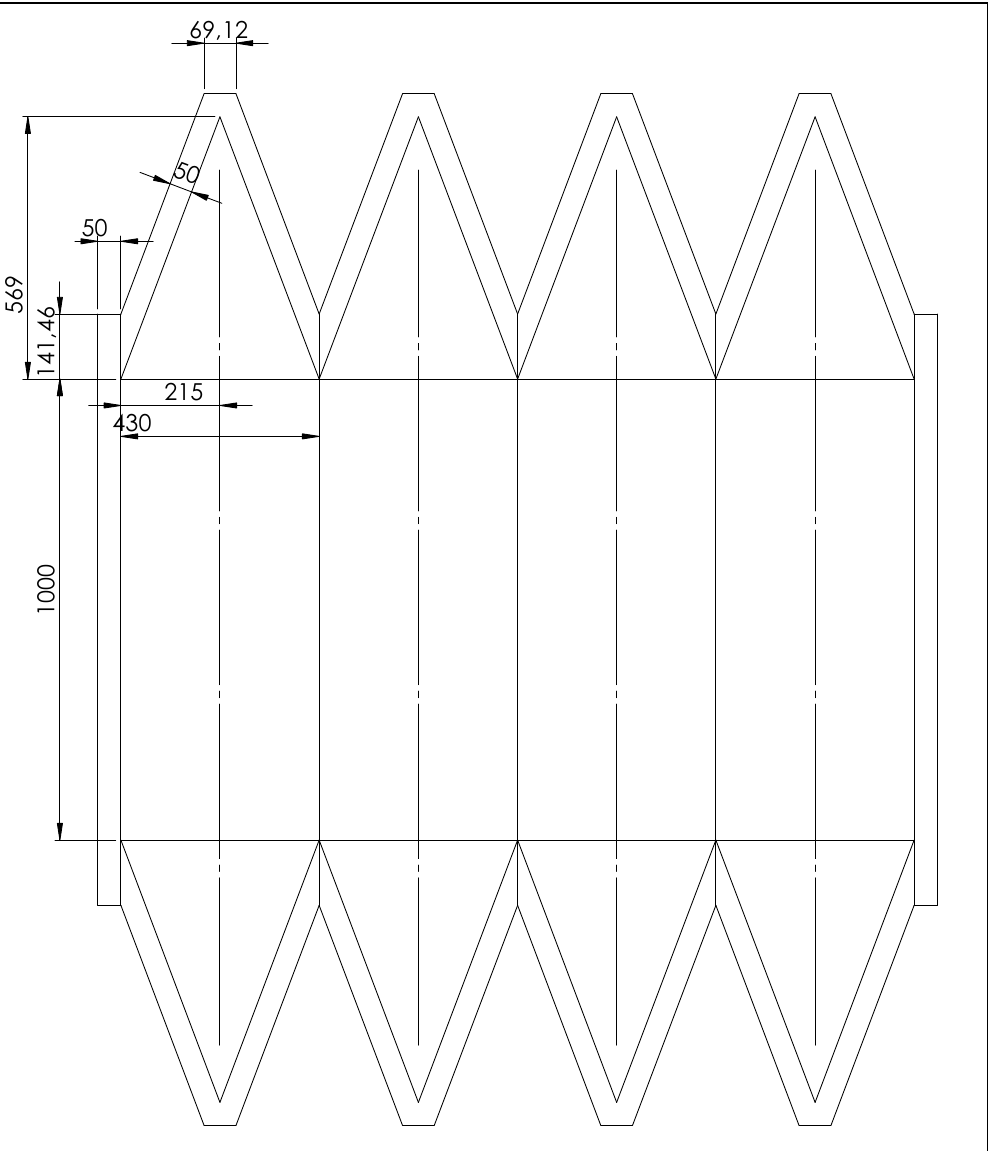
\includegraphics[width=10cm]{../Images/plan_ballon.png}
\end{center}


\subsection{Remplissage}

Le remplissage des ballons se fait par l'usage d'une valve de roue de vélo, cette valve est la plus légère pour l'usage de faibles pressions et possède un clapet anti-retour. D'autre solutions étaient d'utiliser une valve standard pour air comprimé, mais celles ci étaient bien trop lourdes.

La valve de vélo est découpée en laissant un rond de caoutchouc autour pour faciliter le collage sur le PET. Elle est collée sur une des faces les plus longue du parallélépipède et non sur une bordure de collage car elle pourrait créer des plis et donc de potentielles fuites.

\begin{figure}[H]
  \centering
  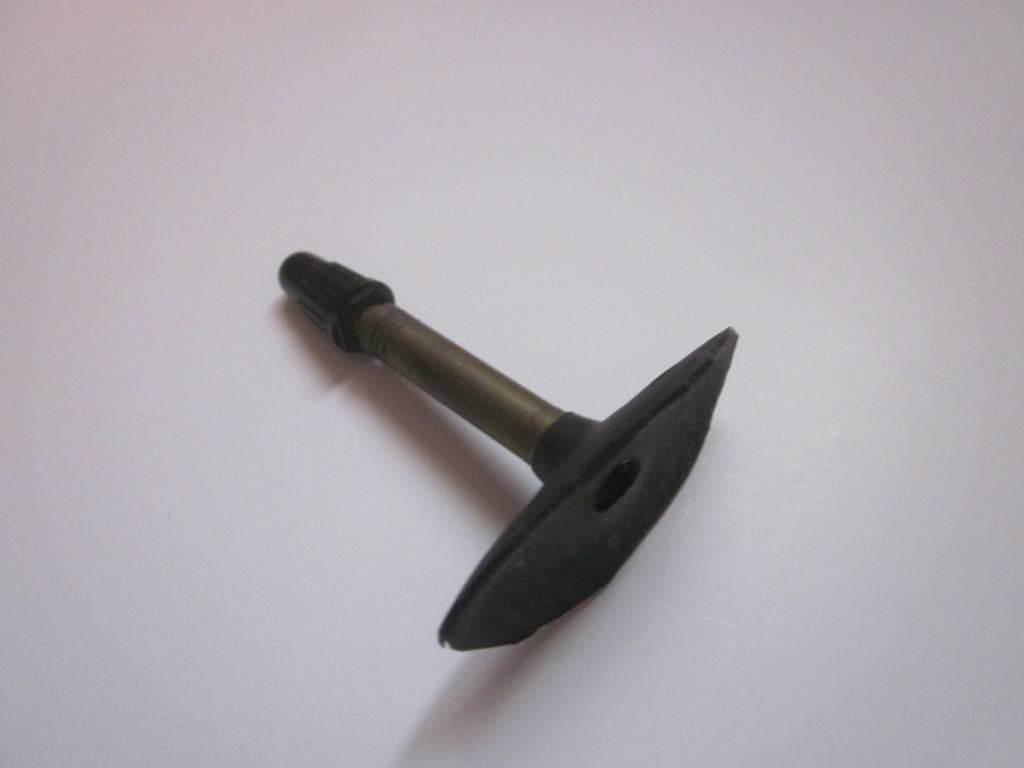
\includegraphics[width=5cm]{../Images/valve.JPG}
  \caption{Valve de remplissage des ballons.}
\end{figure}

\section{Structure}

\subsubsection{Étude des mouvements}

Les 4 moteurs du drone lui confèrent 3 axes de liberté, une de nos contraintes était de permettre de sauvegarder ces libertés pour perdre un minimum de liberté de mouvement, pour cela nous avons choisi une structure triangulaire. Dans cette structure, le centre de gravité du drone est le même que le centre de gravité du ballon, ce qui permet de contrôler le Tropodrone dans toutes les directions. Cette structure permet d'optimiser le nombre de ballons (3) nécessaires pour avoir une pénétration uniforme dans l'air quelque soit la direction prise par le drone.

Le premier modèle a été conçu pour recréer artificiellement les 3 axes de liberté au moyen de disques tournant sur eux-mêmes et autour les uns des autres. Les pièces de liaison ont été réalisées sous Solidworks et imprimées en 3D.

\begin{figure}[H]
 \centering
 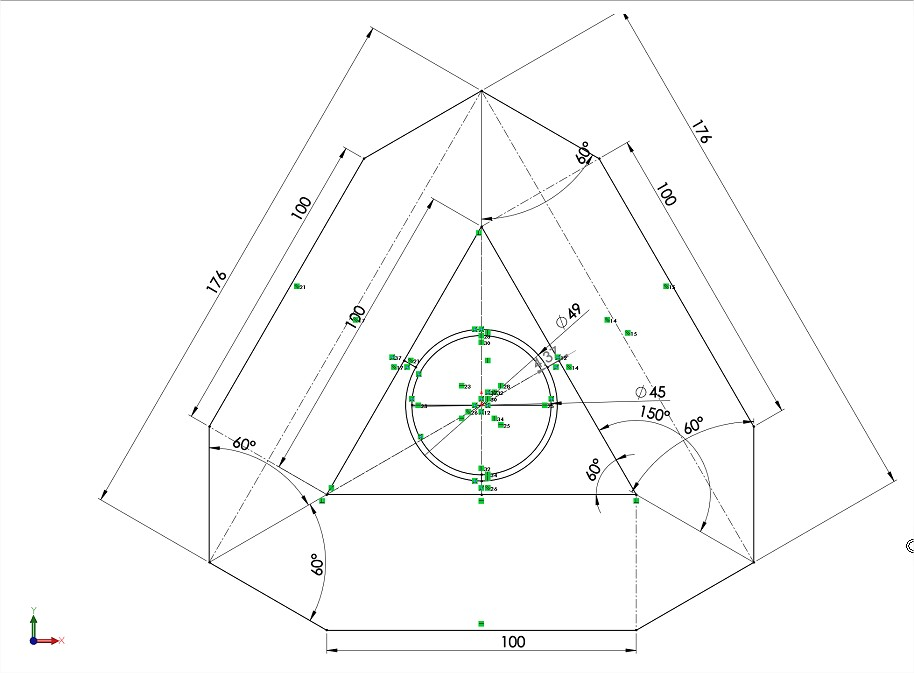
\includegraphics[width=10cm]{../Images/structure0_0.jpg}
 \caption{Premier modèle de la structure.}
 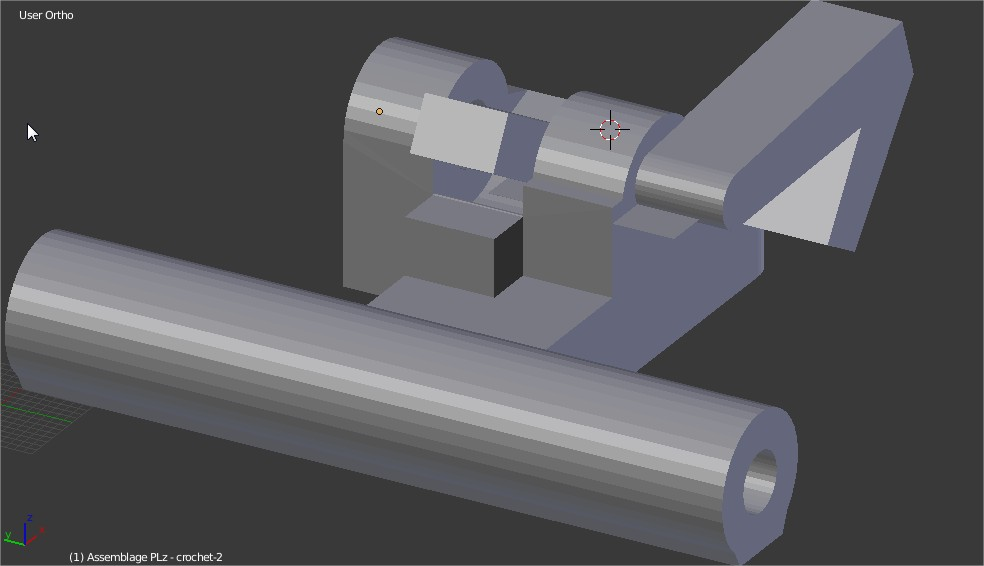
\includegraphics[width=7cm]{../Images/fixation.jpg}
 \caption{Pièce de liaison du premier modèle.}
\end{figure}


Toutefois, ce modèle s'est avéré ne pas être applicable car il était très complexe à mettre en œuvre, nécessitant une modélisation de pièces en 3D complexes, devant en plus être retravaillées après impression et l'ajout de petits roulements pour résoudre des problèmes de frottements des pièces en plastique. Cela aurait augmenté le coût du produit final, sa fragilité et sa complexité. De plus le nombre de pièces à créer rendait la structure trop lourde.

C'est pourquoi nous avons préférés adopter un système plus simple:
Le drone est suspendu par le haut et par le bas par un fil de pèche au centre d'un octaèdre inscrit dans la structure triangulaire des ballons. Cette solution présente les avantages suivants:
\begin{itemize}
	\item simplicité~;
	\item économie, cette solution est moins chère~;
	\item légerté.
\end{itemize}

De plus, elle conserve tous les avantages de la solution précédente:
\begin{itemize}
	\item solidité~;
	\item liberté de mouvement.
\end{itemize}

Nous avons calculé toutes les mensurations de notre structure pour faire des pièces adaptées. Nous avons apporté une attention particulière à l'espace réservé au drone pour qu'il ne percute pas le bord de la structure. Pour que la structure puisse se déformer légèrement afin de laisser le drone pivoter sur lui même, nous avons mis notre hexaèdre en tension vers l'extérieur pour que la structure ne gêne pas le drone en cas de fortes contraintes.

\subsection{Support}

Nous avons modélisé une première version des pièces du support, qui se sont avérés être un peu trop lourde. Nous aurions aimé pouvoir optimiser le design de ces pièces pour obtenir un bien meilleur rapport solidité/poids.

Nous avons également fait un travail de perçage sur nos pièces pour compenser l'imprécision de l'impression 3D.

\subsubsection{Attaches des ballons}

Les ballons doivent être attachés avec une corde se cassant à plus de 230N (voir Chap. contrainte légale).

Étant donné les contraintes du projet, nous avons opté pour des tiges en carbonne, car elles étaient facile à trouver et présentaient un très bon rapport solidité/poids face à d'autres attaches, en métal par exemple. Malheureusement, elles coûtent assez cher (4€ le mètre en moyenne), mais nous avions besoin d'une structure à la fois flexible (pour résister au choc) et rigide (pour le triangle principale, pour éviter les collisions entre le drone et la structure). En jouant sur les tailles des tiges et les versions creuses/pleines, nous avons obtenu le matériel de base de notre structure.

\begin{figure}[H]
	\centering
	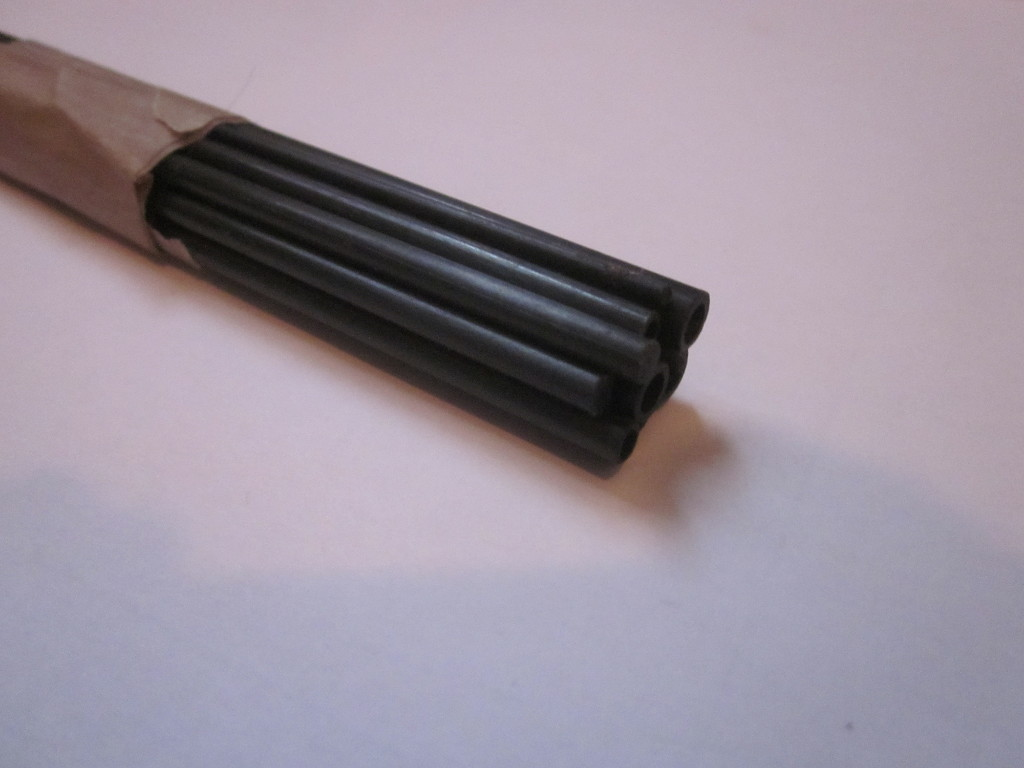
\includegraphics[width=5cm]{../Images/tige_carbone.JPG}
	\caption{Tiges de carbone utilisées.}
\end{figure}


Les quelques recherches que nous avons fait par la suite nous ont mené vers les tiges de carbone, et en particulier les tiges creuses, qui permettent d'allier résistance et faible poids.
La structure est ainsi composée de~:
\begin{itemize}
        \item Tiges de carbone de 6/4mm creuses et pleines
        \item Pièces de liaisons imprimées en 3D
\end{itemize}

\section{Aérodynamisme}
	Notre but a été dans cette partie de chercher une solution technique permettant de réduire la force de traînée que le drone subira quand il se déplacera, et quand il subira l'effet du vent. \\
	Nous répondons ainsi aux contraintes de manoeuvrabilité, en particulier celle lié à la navigation.\\
	Il nous manquait de nombreuses notions en aérodynamisme, que nous avons pû rapidement acquérir grâce au TPE d'élèves de notre classe qui ont fait un remarquable travail sur le sujet, et grâce à un professeur de Prépa qui nous a consacré un peu de son temps.\\
	Nous les remercions ici.
\subsection{Équation de trainée}
	\begin{center}
		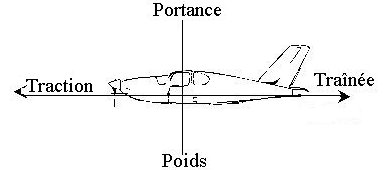
\includegraphics[width=5cm]{../Images/portance.jpg}
		\captionof{figure}{Force de traînée}
	\end{center}
	La force de traînée représente la résistance au mouvement. Elle est matérialisée par l'équation~:\\
  \begin{center}
   \boxed{\displaystyle{F = \frac12 \times \rho \times S \times Cx \times V^2}}
  \end{center}
  Avec~:
  \begin{itemize}
   \item $\rho$ la masse volumique du fluide dans lequel a lieu le déplacement en $kg.m^{-3}$~;
   \item S la surface soumise au flux d'air~;
   \item Cx le coefficient de traînée~;
   \item V la vitesse relative du mobile par rapport au fluide en $m.s^{-1}$.
  \end{itemize}

\subsection{Optimisations techniques}
\subsubsection{Problème des ballons}
	3 ballons de 0.25 m³ créent une surface soumise au flux d'air conséquente, ce qui influe directement sur la force de traînée, la surface S étant un facteur direct.\\
	De plus, suivant la position des ballons, le coefficient de traînée Cx sera plus ou moins conséquent.\\
	\\
	Il nous faut donc trouver une forme favorable, c'est à dire réduisant la surface et ayant un faible coefficient de traînée.\\
	\\
	La réduction du coefficient Cx est difficile à mettre en oeuvre. Elle implique en effet un profil et un angle d'attaque qu'il est difficile de réaliser, notamment par rapport au volume des ballons.\\
	C'est pourquoi nos efforts se sont concentrés sur la réduction de la surface rencontrée.

\subsubsection{La forme en triangle}
	La forme en triangle que nous vous avons présenté précédemment (voir chapitre sur la structure) présente de nombreux avantages.
	\\
	Le premier est qu'elle permet de créer un couloir dans lequel le vent s'engouffre. Ce couloir permet de réduire la force de traînée en limitant la surface des ballons offerte au vent. \\
	Le second avantage est que cette forme ne présente aucune position dans laquelle le vent aurait un trop grand effet.\\
	De plus, nous avons trouvé une solution technique permettant de profiter de ce couloir d'air le plus souvent possible : installer un gouvernail.
\subsubsection{Gouvernail}
	\begin{center}
		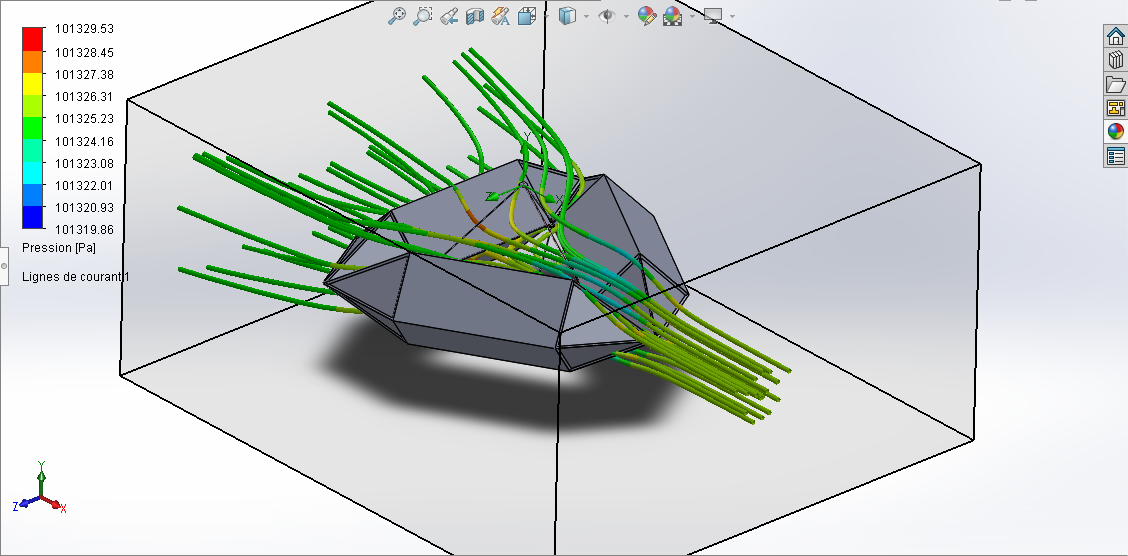
\includegraphics[width=14cm]{../Images/Capture.PNG}
	\end{center}
	Le gouvernail nous permet d'orienter les ballons en fonction de la direction du drone, ce qui force la structure à garder une position théoriquement plus favorable que les autres.
	Nous pouvons faire une analogie avec les différentes conformations d'une molécule : le gouvernail nous permet de garder la position la moins dépensière d'énergie.\\
	\begin{center}
		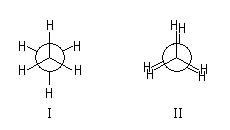
\includegraphics[width=10cm]{../Images/conformations.png}
		\captionof{figure}{Les molécules dépensent moins d'énergie lorsqu'elles sont dans une conformation stable}
	\end{center}
  Cette solution a toutefois un désavantage : elle réduit la manœuvrabilité immédiate du drone en faisant apparaître une force supplémentaire. Toutefois, nos calculs montreront que cette force est négligeable en comparaison du gain sur de longues distances.

\subsection{Calcul du Cx}
	Nous avons dans un premier temps essayé de calculer le Cx à la main, en prenant la seule approximation dont nous avions les données : le Cx d'une sphère.
\subsubsection{Pour une sphère}
\paragraph{Nombre de Reynolds}
	Le coefficient de traînée d'une sphère se calcule en fonction du nombre de Reynolds, qui définit le type d'écoulement auquel est soumis la structure~:


\paragraph{Formule}
	\begin{center}
   \boxed{\displaystyle{Re = \frac{V \times L}{\nu}}}
  \end{center}
	Avec~:
  \begin{itemize}
	 \item $\rho$ la masse volumique du fluide dans lequel a lieu le déplacement en $kg.m^{-3}$~;
   \item V la vitesse relative du mobile par rapport au fluide en $m.s^{-1}$;
   \item L la dimension caractéristique (ici le diamètre de la sphère)~;
   \item $\micro$ la viscosité cinématique du fluide~;
  \end{itemize}

\paragraph{Influence sur les courants créés}
	\begin{center}
		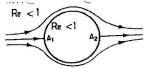
\includegraphics[width=5cm]{../Images/re0.jpg}
		\captionof{figure}{Re < 1}
	\end{center}
	Quand Re < 1, le flux suit un écoulement de Stokes. L'air s'écoule de façon rectiligne.
	\begin{center}
		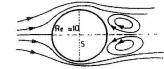
\includegraphics[width=5cm]{../Images/re1.jpg}
		\captionof{figure}{1 < Re < 10³}
	\end{center}
	Quand Re augmente, des tourbillons apparaîssent à l’arrière de la sphère. Ces tourbillons sont à prendre en compte car ils génèrent un courant au centre du support qui augmente la force de traînée.
	\begin{center}
		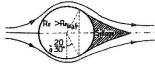
\includegraphics[width=5cm]{../Images/re2.jpg}
		\captionof{figure}{Re > 10³}
	\end{center}
	Quand Re augmente encore, il se crée un sillage qui supprime les tourbillons.\\
	Toutefois, il faut que le flux ait une certaine vitesse pour qu'il se crée un sillage perceptible.\\
	\\
	On comprend bien que le type d'écoulement va considérablement influencer la force de traînée.


\subsubsection{Calculs et limites}
	Nous avons réalisé grâce à cette formule un algorithme python permettant de calculer la force de traînée du ballon.\\
	\lstset{language={Python}}
	\lstinputlisting{../Aerodynamisme/Programmes/calculTrainee.py}
	Toutefois, ce calcul restant une très grosse approximation, nous nous sommes rabattus sur Solidworks et sur son module complémentaire FlowSimulation pour avoir un résultat plus précis.
\subsubsection{Simulation SW}
	L'avantage de Solidworks est que le flux d'air généré pour les calculs épouse parfaitement la forme de la structure, ce qui nous permet d'avoir un résultat bien plus fiable. De plus, il rend possible la quantification du gain promis par le gouvernail.\\
	\begin{center}
		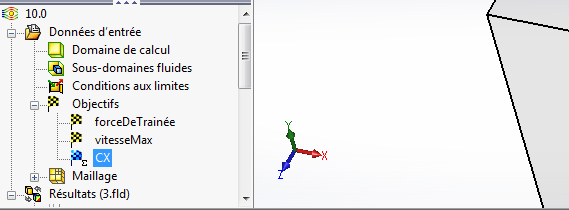
\includegraphics[width=15cm]{../Images/objectifsSW.png}
		\captionof{figure}{Objectifs de calcul.}
	\end{center}
	\begin{center}
		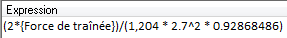
\includegraphics[width=10cm]{../Images/expressionCX.png}
		\captionof{figure}{Expression de Cx dans Solidworks.}
	\end{center}

\subsection{Simulation tableur et équation}
	La simulation a été réalisée plusieurs fois dans plusieurs positions selon l'axe Z.\\
	Ces données ont été rentrées dans un tableur, et nous ont permis de confirmer l'intérêt du gouvernail.\\
	\begin{center}
    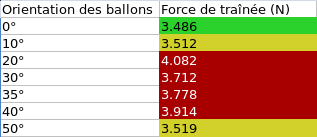
\includegraphics[width=10cm]{../Images/resultatsSW.png} \\
	\end{center}

\subsection{Vitesse du vent maximum}
Pour déterminer la vitesse du vent maximale pouvant être atteinte, il faut se pencher sur les caractéristiques du drone, et en particulier sur la force de traction générée par les moteurs~:\\
Un moteur crée au maximum une force de 4.3 Newtons~; ce qui fait que le drone tout entier (avec les 4 Moteurs) crée une force de traction de 17.2 Newtons.\\
\\
Il faut faire un peu de trigonométrie~:
\begin{center}
	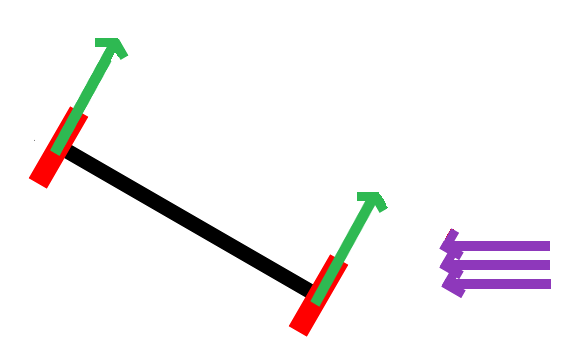
\includegraphics[width=10cm]{../Images/vitesseVent.png}
	\captionof{figure}{Schéma de la situation.}
\end{center}
Les moteurs (en rouge) génèrent une force de traction (en vert) qui est décalée de 60° par rapport au vent (en violet).\\
\\
$A = cos(60) \times 17.2$\\
$A = 8.6 N$\\
Nous avons donc une force de 8.6 N.\\
\\
Après avoir simulé à différentes vitesses, nous trouvons une résistance maximale de 34 $km.h^{-1}$.\\
Le drone peut donc résister à un vent de 34 $km.h^{-1}$.

\newpage

\section{Réalisation}

Nous avons en premier lieu assemblé des ballons aux échelles 1/5 et 1/2. Ceux ci utilisaient de la néoprène car les bordures de collages étaient très courtes dans la longueur. Il nous suffisait d'appliquer la colle, de la laisser sécher puis de presser.

\begin{figure}[H]
 \centering
 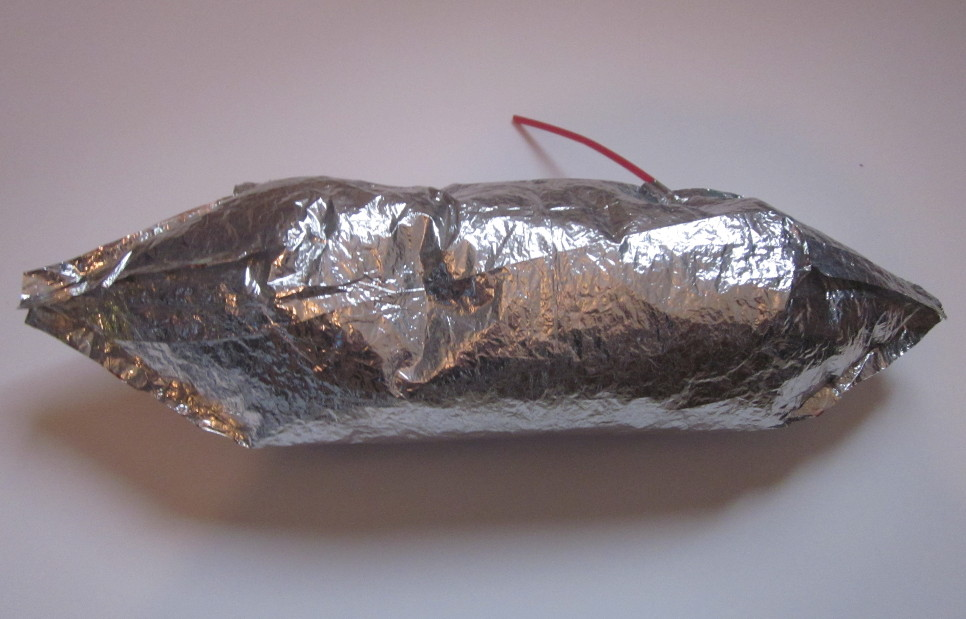
\includegraphics[width=10cm]{../Images/ballon4.JPG}
 \caption{Modèle à l'échelle 1/5 d'un ballon.}
\end{figure}

\subsection{Protocole}

Le protocole d'assemblage trouvé lors de l'assemblage du premier ballon final est le suivant~:
\begin{itemize}
 \item coller de l'adhésif double face sur une planche d'une longueur de plus de 2m (longueur des feuilles de PET)~;
 \item polluer l'adhésif si celui ci est trop adhérent et empêche de décoller correctement le PET~;
 \item presser une feuille de PET sur le bord de l'adhésif~;
 \item nettoyer les surfaces de PET avec de l'acétone pour enlever le revêtement jaune gênant au collage~;
 \item appliquer la colle 401 sur la feuille de PET posée sur l'adhésif le plus proche du bord de la feuille~;
 \item étaler très rapidement à l'aide d'une petit spatule la colle, il faut que celle ci déborde légèrement lors du pressage~;
 \item presser la deuxième feuille de PET sur la première~;
 \item décoller l'ensemble de l'adhésif sans détériorer le collage~;
 \item appliquer de la colle acrylique autour le long de la bordure de collage~;
 \item percer un trou dans le PET de diamètre 8mm avec un emporte pièce~;
 \item appliquer la colle 401 autour du trou~;
 \item presser une valve à travers le trou~;
 \item appliquer de la colle acrylique autour du trou~;
 \item mesurer et tracer le patron de découpe~;
 \item découper le patron avec un cutter en coupant toujours vers l'extérieur du patron pour éviter les déchirements du PET~;
 \item recommencer le procédé de collage pour chacune des jointures.
\end{itemize}

\newpage

\section{Conclusion}

\paragraph{}Ce projet était parti d'une idée un peu folle, mais surtout originale. Nous voulions comprendre et essayer de fabriquer ce modèle de drone que nous désirions vour voler un jour dans le ciel, pour affiner nos compétences techniques et notre maitrise de la gestion d'un projet. Nous avons tous beaucoup appris, que ce soit dans les nombreux domaines scientifiques parcourus ou dans notre expérience gagnée au contact de la réalisation et du concret. Pour nous tous, ce fut une expérience riche d'enseignements qui laissera des souvenirs de nos premières expériences.\\

\paragraph{}Pour conclure, nous remercions nos professeurs de science de l'ingénieur qui nous ont aidés à mener ce projet le plus loin possible. Nous nous remercions également mutuellement pour avoir accompli ce travail jusqu'au bout et sans qu'aucun d'entre nous n'ai jamais été laissé derrière. Et enfin nous vous remercions vous, qui avez pris la peine de lire ce document jusqu'au bout.

\newpage

\section{Images Annexes}

\begin{center}
	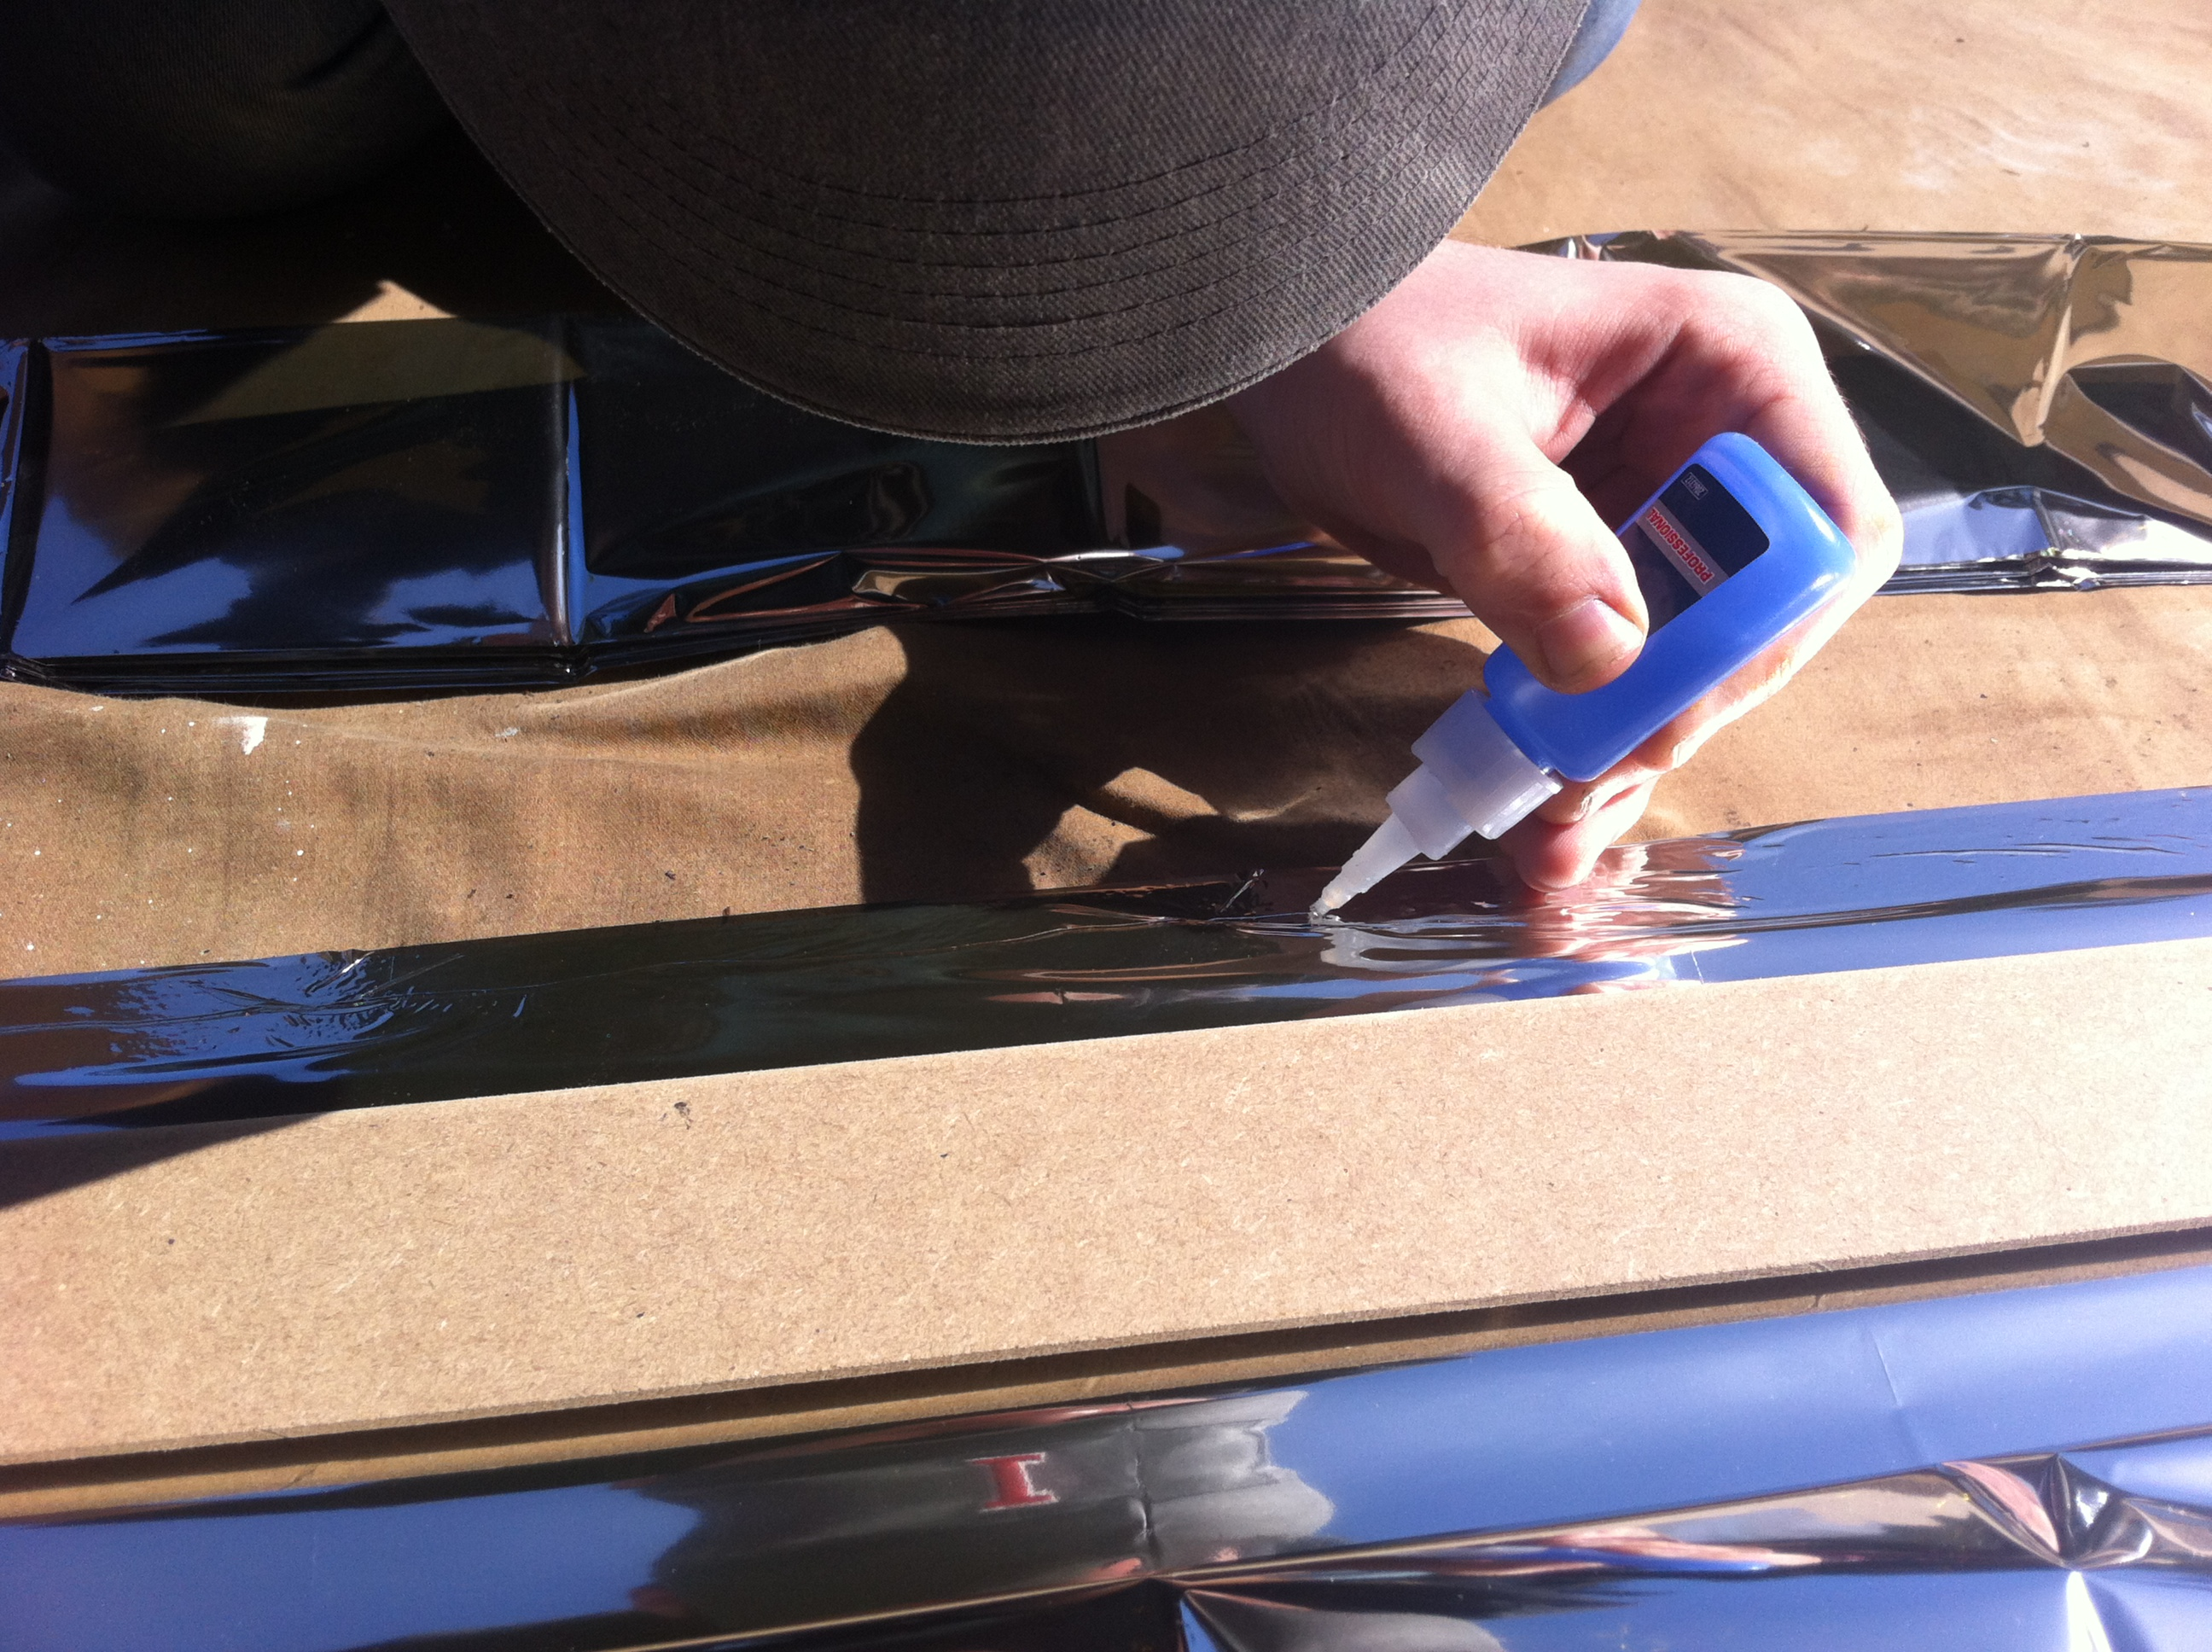
\includegraphics[width=15cm]{../Images/assen_1.JPG}
\end{center}
\begin{center}
	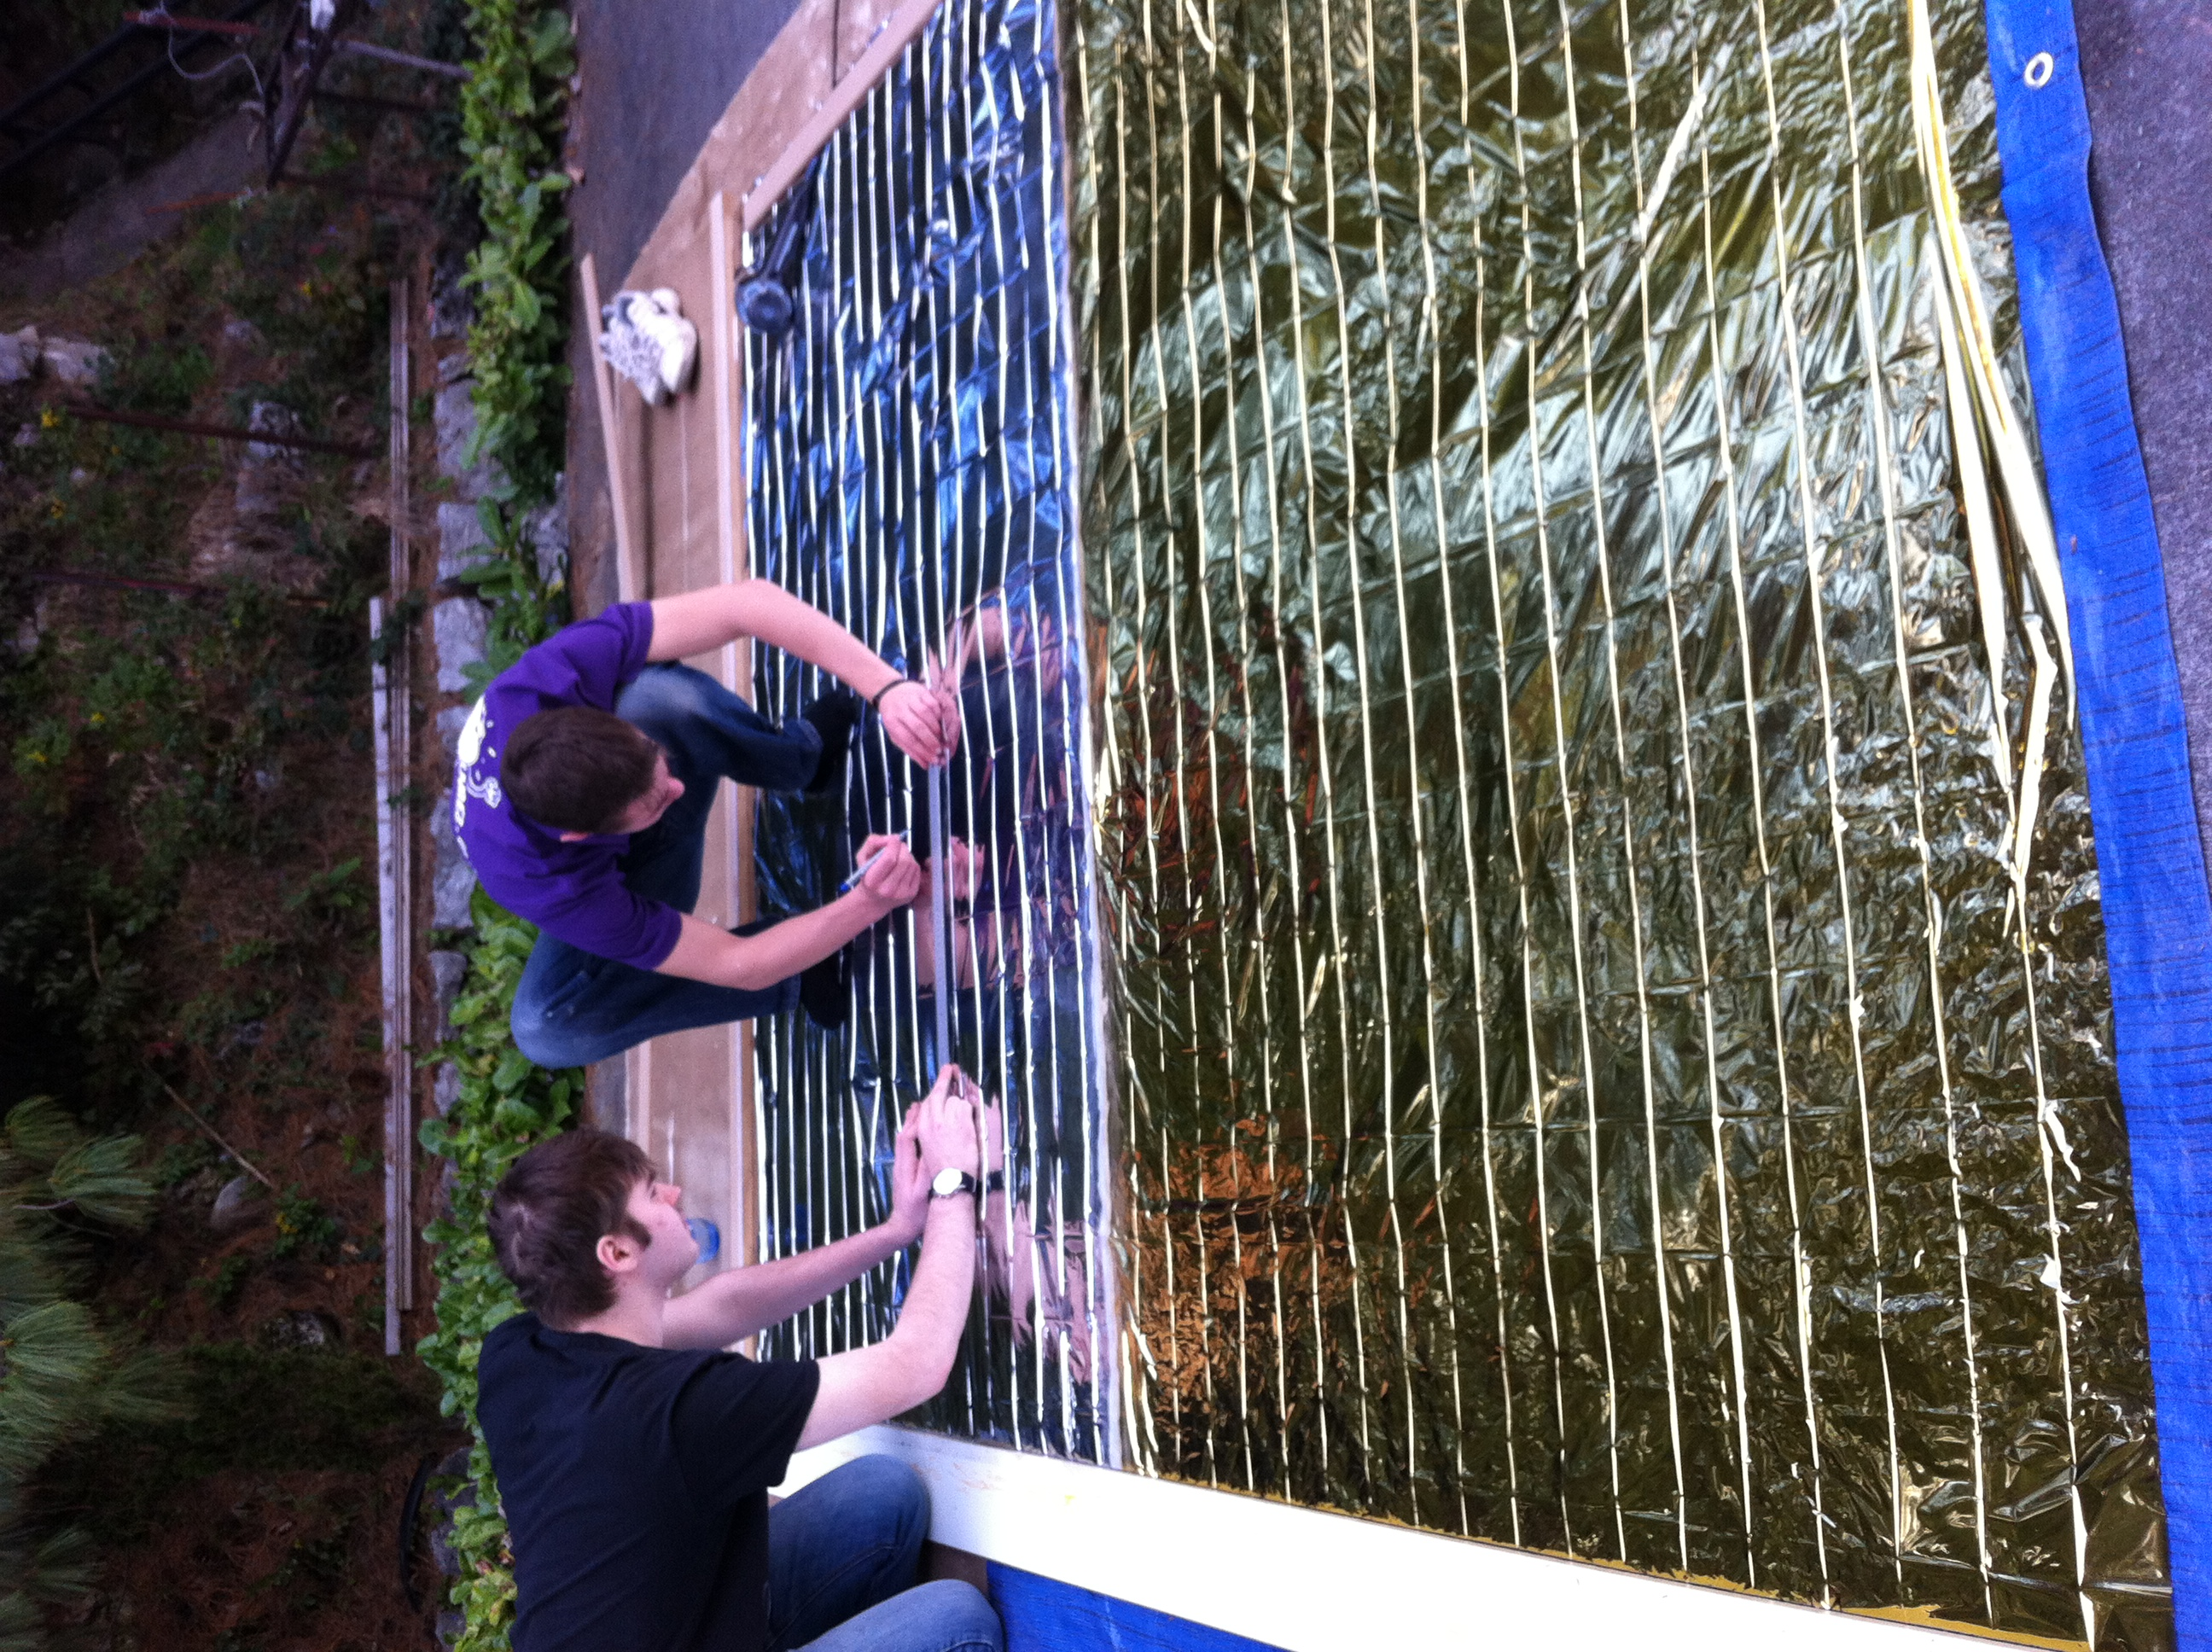
\includegraphics[width=15cm]{../Images/assen_2.JPG}
\end{center}
\begin{center}
	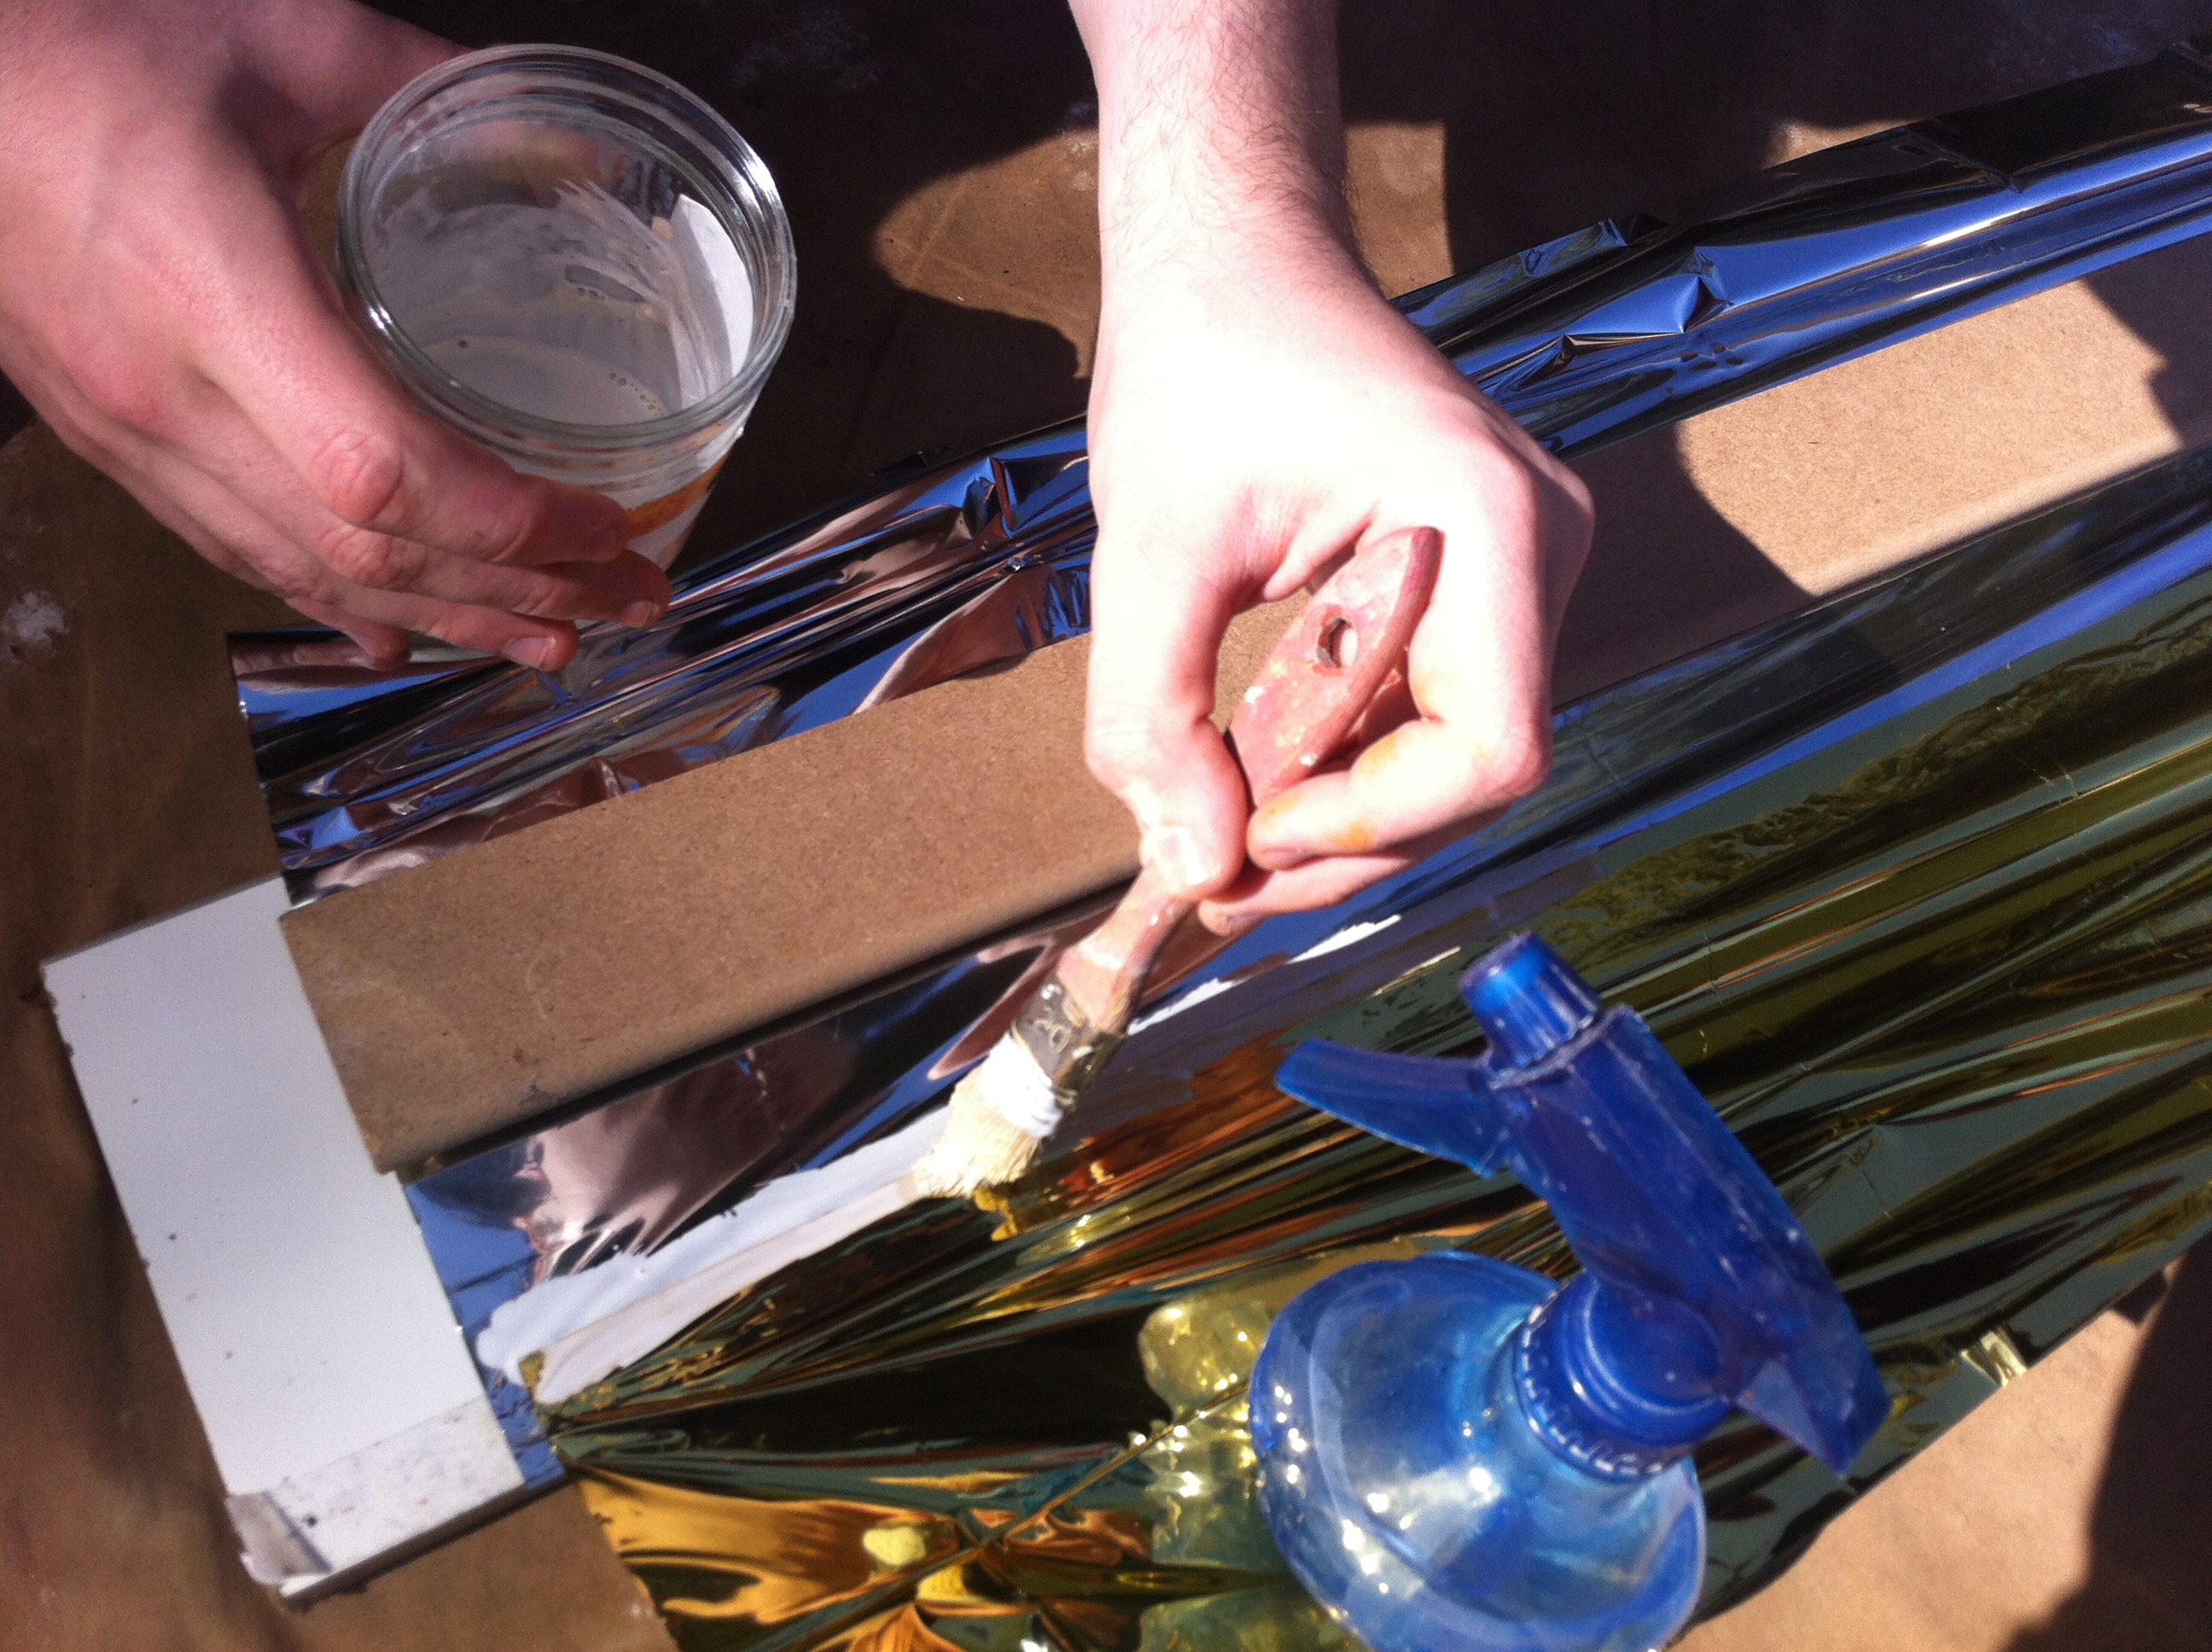
\includegraphics[width=15cm]{../Images/assen_3.JPG}
\end{center}

\section{Références}
\begin{itemize}
  \item \emph{https://media-pim.group-iph.com/medias/products/09/14/8824090001409/technicaldatasheet-fr0.pdf?v=170116093857+0100?attachment=true}
  \item \emph{$https://fr.wikipedia.org/wiki/Pouss\%C3\%A9e_d\%27Archim\%C3\%A8de$}
  \item \emph{http://meteophysique.free.fr/pousse.htm}
  \item \emph{$https://fr.wikipedia.org/wiki/Hydrog\%C3\%A8ne$}
  \item \emph{$https://fr.wikipedia.org/wiki/H\%C3\%A9lium$}
  \item \emph{$https://fr.wikipedia.org/wiki/Loi_de_Charles$}
  \item \emph{$http://aeroballongaz.chez-alice.fr/Enveloppe2.htm$}
  \item \emph{$http://www.airshoot-technologie.com/contents/fr/d38_ballons-photos-helium.html$}
  \item \emph{$http://ballonsolaire.pagesperso-orange.fr/reglementation4m.htm$}
  \item \emph{$http://www.doganak.com/wp-content/uploads/2014/07/Mylar-850.pdf$}
%   \item \emph{}
\end{itemize}

\end{document}
